% Edit only the text between matching begin and end lines.
\documentclass[11pt,a4paper]{article}
% Shared preamble for TMUA worked solutions. Local edits here are overwritten.

% Reproducible PDFs: no timestamps, no trailer id, no build-path details.
\ifdefined\pdfsuppressptexinfo
  \pdfsuppressptexinfo=-1
  \pdfinfoomitdate=1
  \pdftrailerid{}
\fi

\usepackage{graphicx}
\usepackage{mathtools}
\usepackage{amssymb}
\usepackage{amsmath}
\usepackage{amsthm}
\usepackage{enumitem}
\usepackage{microtype}
\usepackage[table]{xcolor}
\usepackage{array}
\usepackage{booktabs}
\usepackage{tabularx}
\usepackage{longtable}
\usepackage{ragged2e}
\usepackage{fancyhdr}
\usepackage{etoolbox}
\usepackage[
  a4paper,
  left=0.8in,
  right=1in,
  top=1in,
  bottom=0.5in,
  headheight=14pt,
  headsep=0.4in
]{geometry}

\usepackage{pgfplots}
\pgfplotsset{compat=1.18}
\usepgfplotslibrary{fillbetween, polar}
\usetikzlibrary{calc, positioning}
\usetikzlibrary{angles, quotes}
\usetikzlibrary{arrows.meta}
\usetikzlibrary{decorations.pathreplacing, decorations.markings}
\usetikzlibrary{patterns}
\usetikzlibrary{intersections}

\usepackage{tocloft}
\usepackage[hidelinks]{hyperref}
\hypersetup{pdfauthor={danieljsmith.org}, pdfcreator={}, pdfsubject={}, pdfkeywords={}}
\urlstyle{same}
\tocloftpagestyle{djssolutions}
\setlength{\cftbeforesubsecskip}{2pt}
\setlength{\cftsubsecindent}{1.5em}
\setlength{\cftsubsecnumwidth}{0pt}
\renewcommand{\cftsubsecfont}{\small\color{black}}
\renewcommand{\cftsubsecpagefont}{\small\color{black}}
\renewcommand{\cftsubsecleader}{\hfill}

% `most` carries the breakable and enhanced libraries the solution box needs.
\usepackage[most]{tcolorbox}
\definecolor{scarlet}{RGB}{205, 40, 75}

\setlength{\parindent}{0pt}

% \djsSolutionsSetup{<paper title>}, called once after this file.
\newcommand{\djsSolnPaperTitle}{}
\newcommand{\djsSolutionsSetup}[1]{%
  \hypersetup{pdftitle={#1 Solutions}}%
  \renewcommand{\djsSolnPaperTitle}{#1}}

% \djsTitleSetup{<booklet>}{<title>}{<paper name>}{<questions>}{<minutes>},
% called once after the setup line, sets the title block that opens the
% contents page, as on the question paper: TMUA and the booklet in spaced
% burgundy capitals, the title, a hairline led by the solution box's short
% scarlet rule, then the paper's name with the question count and, when
% given, the time allowed. Its colours are the site's accent, rule and muted
% text colours.
\definecolor{djsBurgundy}{RGB}{118, 59, 67}
\definecolor{djsHairline}{RGB}{216, 213, 205}
\definecolor{djsSlash}{RGB}{170, 166, 158}
\definecolor{djsMuted}{RGB}{96, 101, 106}
\makeatletter
\newcommand{\djs@booklet}{}
\newcommand{\djs@title}{}
\newcommand{\djs@papername}{}
\newcommand{\djs@details}{}
\newcommand{\djs@caps}[1]{\textls[180]{\MakeUppercase{#1}}}
\newcommand{\djs@dot}{\hspace{0.45em}\textperiodcentered\hspace{0.45em}}
\newcommand{\djsTitleSetup}[5]{%
  \renewcommand{\djs@booklet}{#1}%
  \renewcommand{\djs@title}{#2}%
  \renewcommand{\djs@papername}{#3}%
  \renewcommand{\djs@details}{%
    #4~question\ifnum#4=1 \else s\fi
    \ifblank{#5}{}{\djs@dot#5~minutes}}}
\newcommand{\djsContentsTitle}{%
  {\raggedright\color{djsBurgundy}\footnotesize\bfseries
    \djs@caps{TMUA}{\color{djsSlash}\hspace{0.55em}/\hspace{0.55em}}%
    \djs@caps{\djs@booklet}\par}%
  \vspace{7pt}%
  {\raggedright\fontsize{24.88}{28}\selectfont\djs@title\par}%
  \vspace{9pt}%
  \noindent\makebox[0pt][l]{\color{djsHairline}\rule[0.9pt]{\linewidth}{0.6pt}}%
  {\color{scarlet}\rule{3.5cm}{2.2pt}}\par
  \vspace{5pt}%
  {\small\color{djsMuted}\djs@papername\hfill\djs@details\par}%
  \vspace{8pt}}
\makeatother

% The header appears only on the contents page and each question's opening
% page. Continuation pages use the empty default style.
\fancypagestyle{djssolutions}{%
  \fancyhead{}%
  \fancyfoot{}%
  \renewcommand{\headrulewidth}{0.9pt}%
  \fancyhead[L]{\textit{Solutions} - \djsSolnPaperTitle}%
  \fancyhead[R]{\href{https://danieljsmith.org/?utm_source=pdf&utm_campaign=tmua&utm_content=solutions}{danieljsmith.org}}%
}
\pagestyle{empty}

% \djsLastUpdated{<date>}, called once after the setup line: one line
% at the foot of the first page only, left-aligned under the left header at
% the 0.8in left margin. It is drawn over the page rather than set as a
% footer, so no page style changes.
\newcommand{\djsLastUpdated}[1]{%
  \AtBeginDocument{\AddToHookNext{shipout/foreground}{%
    \put(0.8in,-\dimexpr\paperheight-0.32in\relax){\makebox[0pt][l]{%
      \footnotesize Last updated #1}}}}}

\newcolumntype{Y}{>{\RaggedRight\arraybackslash}X}

% Question layout, identical to the question paper's.
\newcommand{\djsTocTopic}[1]{%
  \ifblank{#1}{}{%
    \texorpdfstring
      {\hspace{0.9em}{\footnotesize\itshape\color{black!45}#1}}
      { \textendash\ #1}}}
\newcommand{\djsTopicLine}[1]{%
  \ifblank{#1}{}{%
    {\raggedleft\footnotesize\itshape\color{black!45}#1\par}%
    \vspace{-0.6\baselineskip}}}
\newcommand{\questionitem}[1][]{%
  \item\phantomsection
  \addcontentsline{toc}{subsection}{%
    Question \number\value{enumi}\protect\djsTocTopic{#1}}%
}
\renewcommand{\contentsname}{Questions}
\newcommand{\djsFrontMatter}{%
  \vspace*{6pt}%
  \djsContentsTitle
  \vspace{14pt}%
  \tableofcontents
  \newpage
}

% The solution body: a white breakable box with a left scarlet rule. The
% rule continues onto a continuation page and stops where the solution
% stops, then turns into a short horizontal of the same weight so the
% solution visibly ends. The argument is the answer label.
\newcommand{\djsSolutionAnswer}[1]{%
  {\color{scarlet}\bfseries Answer\ \ #1}}
\newtcolorbox{djsSolution}[1]{%
  enhanced, breakable, frame hidden, sharp corners, colback=white,
  height fixed for=first and middle, height fill,
  extras unbroken and last={natural height},
  borderline west={2.2pt}{0pt}{scarlet},
  left=11pt, right=0pt, top=5pt, bottom=13pt,
  before skip=13pt, after skip=4pt,
  overlay unbroken and last={%
    \fill[scarlet] (frame.south west)
      rectangle ([xshift=3.5cm, yshift=2.2pt]frame.south west);},
  before upper={\setlength{\parskip}{6pt}%
                {\color{scarlet}\bfseries Solution}%
                \hfill\djsSolutionAnswer{#1}\par\vspace{4pt}}}

% Solution figures sit inside the box and are drawn smaller than question
% figures; \scalebox shrinks node text with the drawing.
\newcommand{\SolnFigureScale}{0.85}
\newsavebox{\djsSolnFigureBox}
\newenvironment{djsSolutionFigure}
  {\par\vspace{4pt}\begin{center}\begin{lrbox}{\djsSolnFigureBox}}
  {\end{lrbox}\scalebox{\SolnFigureScale}{\usebox{\djsSolnFigureBox}}%
   \end{center}\vspace{2pt}\par}

\djsSolutionsSetup{TMUA Set B Paper 2}
\djsLastUpdated{30 September 2026}
\begin{document}
\thispagestyle{djssolutions}
\djsFrontMatter
\clearpage
\thispagestyle{djssolutions}
\vspace*{8pt}
\djsTopicLine{Polynomials}
\begin{enumerate}[label=\textbf{\arabic*.},leftmargin=*,itemsep=0pt,start=1]
\questionitem[Polynomials]
% begin q000071 stem
For a real constant $k$, consider the equation \[ x^4-4x^2+k=0 \] Which of the following conditions on $k$ is \textbf{necessary and sufficient} for the equation to have exactly two distinct real solutions?
% end q000071 stem

\par\vspace*{12pt}
\begin{tabularx}{\linewidth}{@{}>{\bfseries}l Y@{}}
A &
% begin q000071 choice A
$k>4$
% end q000071 choice A
\\[0.8em]
B &
% begin q000071 choice B
$k=4$
% end q000071 choice B
\\[0.8em]
C &
% begin q000071 choice C
$k\leq0$
% end q000071 choice C
\\[0.8em]
D &
% begin q000071 choice D
$0<k<4$
% end q000071 choice D
\\[0.8em]
E &
% begin q000071 choice E
$k=0$
% end q000071 choice E
\\[0.8em]
F &
% begin q000071 choice F
$k<0$ or $k=4$
% end q000071 choice F
\\[0.8em]
G &
% begin q000071 choice G
$k<0$
% end q000071 choice G
\\
\end{tabularx}

\begin{djsSolution}{F}
% begin q000071 solution
A condition is necessary if it must hold whenever the equation has exactly two distinct real solutions. It is sufficient if it guarantees exactly two distinct real solutions. We need a condition for which both statements are true.

Put $u=x^2$, so $u\geq0$. The equation becomes
\[
u^2-4u+k=0
\]

Each positive value of $u$ gives two distinct values $x=\pm\sqrt{u}$. The value $u=0$ gives only $x=0$, while a negative value of $u$ gives no real $x$.

For $k\leq4$, the quadratic formula gives
\[
u=\frac{4\pm\sqrt{(-4)^2-4(1)(k)}}{2(1)}
=2\pm\sqrt{4-k}
\]

First, if $k<0$, then $\sqrt{4-k}>2$. Thus $2-\sqrt{4-k}<0$, while $2+\sqrt{4-k}>0$. Only the positive value of $u$ gives real solutions, namely
\[
x=-\sqrt{2+\sqrt{4-k}}\quad\text{or}\quad x=\sqrt{2+\sqrt{4-k}}
\]

If $k=0$, then
\[
u=2\pm\sqrt4=0\quad\text{or}\quad 4
\]
so the three distinct real solutions are
\[
x=-2,\quad 0,\quad 2
\]

If $0<k<4$, then $0<\sqrt{4-k}<2$. Hence $2-\sqrt{4-k}$ and $2+\sqrt{4-k}$ are distinct positive values of $u$, each giving two values of $x$. There are four distinct real solutions.

If $k=4$, the two values given by the quadratic formula coincide:
\[
u=2\pm\sqrt0=2
\]
This repeated value of $u$ still gives exactly two distinct real solutions:
\[
x=-\sqrt2\quad\text{or}\quad x=\sqrt2
\]
Counting the repeated value of $u$ again would not create additional solutions.

Finally, if $k>4$, the discriminant $16-4k$ is negative. There is no real value of $u$, so there is no real value of $x$.

These cases cover every real $k$. If the equation has exactly two distinct real solutions, then $k<0$ or $k=4$; and if $k<0$ or $k=4$, then the equation has exactly two distinct real solutions. The correct option is \textbf{F}.
% end q000071 solution
\end{djsSolution}
\end{enumerate}
\clearpage
\thispagestyle{djssolutions}
\vspace*{8pt}
\djsTopicLine{Number}
\begin{enumerate}[label=\textbf{\arabic*.},leftmargin=*,itemsep=0pt,start=2]
\questionitem[Number]
% begin q000108 stem
Let $n$ be an integer. Consider the following conditions:
\[
\begin{array}{@{}l l@{}}
\textbf{I:} & \text{$n$ is odd} \\[2pt]
\textbf{II:} & \text{$n$ is a multiple of $4$} \\[2pt]
\textbf{III:} & \text{$n$ is a prime greater than $3$}
\end{array}
\]
Which of these conditions is/are \textbf{sufficient} to guarantee that $n^3-n$ is divisible by $12$?
% end q000108 stem

\par\vspace*{12pt}
\begin{tabularx}{\linewidth}{@{}>{\bfseries}l Y@{}}
A &
% begin q000108 choice A
None of them
% end q000108 choice A
\\[0.8em]
B &
% begin q000108 choice B
I only
% end q000108 choice B
\\[0.8em]
C &
% begin q000108 choice C
II only
% end q000108 choice C
\\[0.8em]
D &
% begin q000108 choice D
III only
% end q000108 choice D
\\[0.8em]
E &
% begin q000108 choice E
I and II only
% end q000108 choice E
\\[0.8em]
F &
% begin q000108 choice F
I and III only
% end q000108 choice F
\\[0.8em]
G &
% begin q000108 choice G
II and III only
% end q000108 choice G
\\[0.8em]
H &
% begin q000108 choice H
I, II, and III
% end q000108 choice H
\\
\end{tabularx}

\begin{djsSolution}{H}
% begin q000108 solution
A condition is sufficient if, whenever it holds, $n^3-n$ is divisible by $12$.

Using difference-of-two-squares we can factorise
\begin{align*}
n^3-n&=n(n^2-1)\\[5pt]
&=n(n-1)(n+1)
\end{align*}

The factors $n-1$, $n$ and $n+1$ are three consecutive integers, so one is a multiple of $3$. To make their product divisible by $12$, we also need a factor of $4$.\\

For I, if $n$ is odd, then $n-1$ and $n+1$ are even. They differ by $2$, so one is a multiple of $4$ and the other is twice an odd number. Thus the product has a factor of $4$ as well as a factor of $3$, and I is sufficient.\\

For II, if $n$ is a multiple of $4$, the product already has a factor of $4$ from $n$. It also has a factor of $3$ because its factors are consecutive integers, so II is sufficient.\\

For III, a prime greater than $3$ is odd: the only even prime is $2$. Hence $n-1$ and $n+1$ are even and differ by $2$, so one is a multiple of $4$. The three consecutive factors also supply a multiple of $3$, so III is sufficient.\\

All three conditions are sufficient. The correct option is \textbf{H}.
% end q000108 solution
\end{djsSolution}
\end{enumerate}
\clearpage
\thispagestyle{djssolutions}
\vspace*{8pt}
\djsTopicLine{Polynomials}
\begin{enumerate}[label=\textbf{\arabic*.},leftmargin=*,itemsep=0pt,start=3]
\questionitem[Polynomials]
% begin q000612 stem
The curve $C$ has equation $y=x^3-3x^2$

A tangent to $C$ passes through the point $P(0,1)$. The point at which the tangent touches $C$ has $x$-coordinate $t$

Find the complete set of possible values of $t$
% end q000612 stem

\par\vspace*{12pt}
\begin{tabularx}{\linewidth}{@{}>{\bfseries}l Y@{}}
A &
% begin q000612 choice A
$t=-\frac12$ only
% end q000612 choice A
\\[0.8em]
B &
% begin q000612 choice B
$t=1$ only
% end q000612 choice B
\\[0.8em]
C &
% begin q000612 choice C
$t=-\frac12$ or $t=1$
% end q000612 choice C
\\[0.8em]
D &
% begin q000612 choice D
$t=-1$ or $t=1$
% end q000612 choice D
\\[0.8em]
E &
% begin q000612 choice E
$t=\frac12$ or $t=1$
% end q000612 choice E
\\[0.8em]
F &
% begin q000612 choice F
$t=-\frac12$ or $t=\frac32$
% end q000612 choice F
\\
\end{tabularx}

\begin{djsSolution}{C}
% begin q000612 solution
Differentiate to find the gradient of the tangent at $x=t$:
\[
\frac{\mathrm{d}y}{\mathrm{d}x}=3x^2-6x
\]

The tangent has gradient $3t^2-6t$ and touches $C$ at $(t,t^3-3t^2)$. The point $P$ lies on the tangent, not necessarily on $C$, so its $x$-coordinate $0$ is not $t$.

The equation of a line through $(x_1,y_1)$ with gradient $m$ is $y-y_1=m(x-x_1)$. Substituting the point of contact and the gradient gives
\[
y-(t^3-3t^2)=(3t^2-6t)(x-t)
\]

Since the tangent passes through $P(0,1)$, put $x=0$ and $y=1$:
\[
1-(t^3-3t^2)=(3t^2-6t)(0-t)
\]

Expanding,
\[
1-t^3+3t^2=-3t^3+6t^2
\]

Rearranging,
\[
2t^3-3t^2+1=0
\]

The choices repeatedly suggest $t=1$, so try it first:
\[
2(1)^3-3(1)^2+1=0
\]

By the factor theorem, if a polynomial is zero at $t=a$, then $t-a$ is a factor. Thus $t-1$ is a factor here. 

Polynomial division by $t-1$ obtains
\[
2t^3-3t^2+1
=(t-1)(2t^2-t-1)
\]

Factorising the quadratic in the usual way gives $2t^2-t-1=(t-1)(2t+1)$. Hence the equation becomes
\[
(t-1)^2(2t+1)=0
\]

Therefore the complete set of possible values is
\[
t=1\quad\text{or}\quad t=-\frac12
\]

Although $t-1$ appears twice, it gives only one value of $t$. The correct option is \textbf{C}.
% end q000612 solution
\end{djsSolution}
\end{enumerate}
\clearpage
\thispagestyle{djssolutions}
\vspace*{8pt}
\djsTopicLine{Algebra}
\begin{enumerate}[label=\textbf{\arabic*.},leftmargin=*,itemsep=0pt,start=4]
\questionitem[Algebra]
% begin q000016 stem
A student is required to solve the equation \[ 3\sqrt{x+1}=x-1 \]

Their attempt is as follows:

\[ \begin{aligned} 3\sqrt{x+1}=x-1 &\xRightarrow{\textbf{(I)}} 9(x+1)=(x-1)^2\\[10pt] 9(x+1)=(x-1)^2 &\xRightarrow{\textbf{(II)}} 9x+9=x^2-2x+1\\[10pt] 9x+9=x^2-2x+1 &\xRightarrow{\textbf{(III)}} x^2-11x-8=0\\[10pt] x^2-11x-8=0 &\xRightarrow{\textbf{(IV)}} x=\dfrac{11\pm 3\sqrt{17}}{2} \\[10pt] \end{aligned} \] They then conclude that the solutions of the original equation are $x=\dfrac{11+3\sqrt{17}}{2}$ and $x=\dfrac{11-3\sqrt{17}}{2}$. Which one of the following is true?
% end q000016 stem

\par\vspace*{12pt}
\begin{tabularx}{\linewidth}{@{}>{\bfseries}l Y@{}}
A &
% begin q000016 choice A
The solution is correct.
% end q000016 choice A
\\[0.8em]
B &
% begin q000016 choice B
Only one of $x=\dfrac{11+3\sqrt{17}}{2}$ and $x=\dfrac{11-3\sqrt{17}}{2}$ is correct and the error arises as a result of step (I).
% end q000016 choice B
\\[0.8em]
C &
% begin q000016 choice C
Only one of $x=\dfrac{11+3\sqrt{17}}{2}$ and $x=\dfrac{11-3\sqrt{17}}{2}$ is correct and the error arises as a result of step (II).
% end q000016 choice C
\\[0.8em]
D &
% begin q000016 choice D
Only one of $x=\dfrac{11+3\sqrt{17}}{2}$ and $x=\dfrac{11-3\sqrt{17}}{2}$ is correct and the error arises as a result of step (III).
% end q000016 choice D
\\[0.8em]
E &
% begin q000016 choice E
There is another value of $x$ that satisfies the original equation and the error arises as a result of step (I).
% end q000016 choice E
\\[0.8em]
F &
% begin q000016 choice F
There is another value of $x$ that satisfies the original equation and the error arises as a result of step (II).
% end q000016 choice F
\\[0.8em]
G &
% begin q000016 choice G
There is another value of $x$ that satisfies the original equation and the error arises as a result of step (III).
% end q000016 choice G
\\
\end{tabularx}

\begin{djsSolution}{B}
% begin q000016 solution
When an attempt produces proposed solutions, substituting them back into the original equation is often a useful first move, before studying the steps. 

Substituting these surds exactly looks tedious, but $\sqrt{17}\approx4$ gives quick estimates:
\[
\begin{aligned}
\frac{11-3\sqrt{17}}{2}&\approx\frac{11-3(4)}{2}=-\frac12 = 0.5\\[8pt]
\frac{11+3\sqrt{17}}{2}&\approx\frac{11+3(4)}{2}=\frac{23}{2}=11.5\\
\end{aligned}
\]

The minus-sign root $\approx 0.5$ is below $1$, so the right hand side $x-1$ of the original equation is negative for this value of $x$. Meanwhile, the left hand side of the original equation is always positive, a contradiction.

Therefore, without directly substituting, we can realise that the negative root
\[ x = \frac{11-3\sqrt{17}}{2} \]

is not a valid solution. This points us towards B, C or D and indicates we should look for a step where extra solutions were introduced.

Now lets look at the solution itself. Starting with Step I:

Squaring both sides is a valid forward step, but the squared equation need not give only solutions of the original equation. 

In general, squaring both sides of an equation of form $a=b$ obtains $a^2=b^2$. But the solutions of $a^2=b^2$ include both the solutions of $a=b$ \textbf{and} $a=-b$, so the solutions must be checked before they are claimed to solve $a=b$ specifically. For example, $a=1$ and $b=-1$ give $a^2=b^2$, although $a\ne b$.

The correct answer is therefore \textbf{B}. 

Squaring both sides in Step I introduced the extraneous solution \[x=\frac{11-3\sqrt{17}}{2}\] 
which does not solve the original equation. \\[5pt]

\textit{Remark:}

In this context, the positive root 
\[x=\frac{11+3\sqrt{17}}{2}\]

solve the original equation
\[ 3\sqrt{x+1}=x-1 \]

whilst the negative root 
\[x=\frac{11-3\sqrt{17}}{2}\]

solves the original equation with negated right hand side
\[ 3\sqrt{x+1}=-x+1 \]

Whilst not necessary to answer the question, we can directly verify that the subsequent steps are all valid. 

Step II is a correct expansion of brackets. Step III is a correct collection of like terms. Step IV is a correct application of the quadratic formula:
\[
\begin{aligned}
x&=\frac{-(-11)\pm\sqrt{(-11)^2-4(1)(-8)}}{2(1)}\\[8pt]
&=\frac{11\pm\sqrt{153}}{2}\\[8pt]
&=\frac{11\pm3\sqrt{17}}{2}
\end{aligned}
\]
Step IV is correct: but these are the two solutions of the \emph{squared} equation, not the original equation.
% end q000016 solution
\end{djsSolution}
\end{enumerate}
\clearpage
\thispagestyle{djssolutions}
\vspace*{8pt}
\djsTopicLine{Trigonometry}
\begin{enumerate}[label=\textbf{\arabic*.},leftmargin=*,itemsep=0pt,start=5]
\questionitem[Trigonometry]
% begin q000063 stem
Let $p$ be a real constant. Consider the equation \[\sin x \cos x = p\] on $0 \le x < 2\pi$

Which of the following statements is/are true? \[ \begin{array}{@{}l l@{}}
\textbf{I:} & \text{If } |p|<\tfrac12 \text{ then the equation has exactly 4 distinct solutions} \\[5pt]
\textbf{II:} & \text{If the equation has exactly 2 distinct solutions, then } |p|=\dfrac12
\end{array} \]
% end q000063 stem

\par\vspace*{12pt}
\begin{tabularx}{\linewidth}{@{}>{\bfseries}l Y@{}}
A &
% begin q000063 choice A
None of them
% end q000063 choice A
\\[0.8em]
B &
% begin q000063 choice B
I only
% end q000063 choice B
\\[0.8em]
C &
% begin q000063 choice C
II only
% end q000063 choice C
\\[0.8em]
D &
% begin q000063 choice D
I and II
% end q000063 choice D
\\
\end{tabularx}

\begin{djsSolution}{D}
% begin q000063 solution
The double-angle identity for $\sin(2A)$ is outside the TMUA specification, but it is worth knowing. Students who do not know it should see the alternative solution below, which does not require it.

The identity \[\sin(2A)=2\sin A\cos A\] gives a quick route.

On $0\le 2x<4\pi$, the equation becomes
\[
\sin(2x)=2p
\]

\begin{djsSolutionFigure}
% begin q000063 figure F1
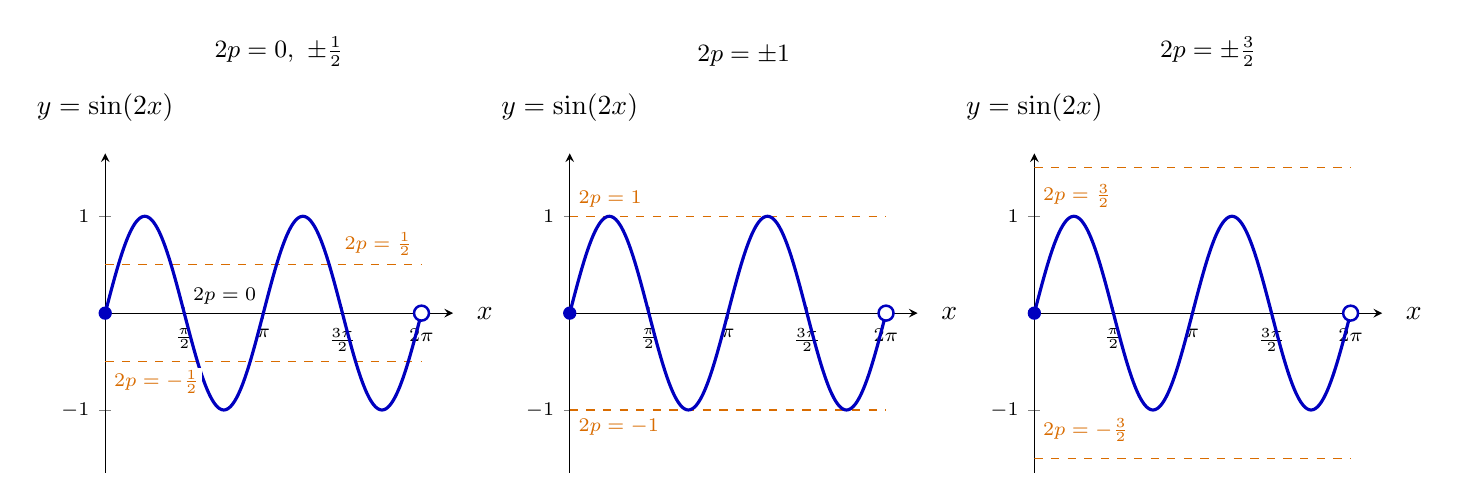
\begin{tikzpicture}
\pgfmathsetmacro{\pival}{pi}
\pgfmathsetmacro{\twopi}{2*pi}
\pgfmathsetmacro{\threepi}{3*pi}
\pgfmathsetmacro{\fourpi}{4*pi}
\pgfplotsset{
  sine panel/.style={
    width=6cm, height=5.64cm,
    xmin=0, xmax=1.1*\fourpi, ymin=-1.65, ymax=1.65,
    axis lines=middle, axis line style={black},
    enlarge x limits=false, enlarge y limits=false,
    xtick={0,\pival,\twopi,\threepi,\fourpi},
    xticklabels={$0$,$\frac{\pi}{2}$,$\pi$,$\frac{3\pi}{2}$,$2\pi$},
    ytick={-1,0,1},
    tick label style={font=\scriptsize},
    xlabel={$x$},
    xlabel style={at={(axis description cs:1.04,0.5)},anchor=west},
    ylabel={$y=\sin(2x)$},
    ylabel style={at={(axis description cs:0,1.07)},anchor=south,rotate=0},
    title style={at={(axis description cs:0.5,1.19)},anchor=south,font=\small},
    clip=true, clip marker paths=false
  }
}
\begin{axis}[sine panel,at={(0cm,0cm)},anchor=south west,
  title={$2p=0,\ \pm\tfrac12$}]
  \addplot[orange!85!black,thin,dashed,domain=0:\fourpi,samples=2] {0.5};
  \addplot[orange!85!black,thin,dashed,domain=0:\fourpi,samples=2] {-0.5};
  \addplot[blue!75!black,line width=1.15pt,domain=0:\fourpi,samples=241]
    {sin(deg(x))};
  \node[anchor=south east,xshift=-2pt,yshift=2pt,font=\scriptsize,
    text=orange!85!black,fill=white,inner sep=1pt]
    at (axis cs:\fourpi,0.5) {$2p=\tfrac12$};
  \node[anchor=north west,xshift=2pt,yshift=-2pt,font=\scriptsize,
    text=orange!85!black,fill=white,inner sep=1pt]
    at (axis cs:0,-0.5) {$2p=-\tfrac12$};
  \node[anchor=south west,xshift=2pt,yshift=2pt,font=\scriptsize,
    fill=white,inner sep=1pt]
    at (axis cs:\pival,0) {$2p=0$};
  \addplot[only marks,mark=*,mark size=2.2pt,blue!75!black]
    coordinates {(0,0)};
  \addplot[only marks,mark=*,mark size=2.7pt,
    mark options={draw=blue!75!black,fill=white,line width=0.9pt}]
    coordinates {(\fourpi,0)};
\end{axis}
\begin{axis}[sine panel,at={(5.9cm,0cm)},anchor=south west,
  title={$2p=\pm1$}]
  \addplot[orange!85!black,thin,dashed,domain=0:\fourpi,samples=2] {1};
  \addplot[orange!85!black,thin,dashed,domain=0:\fourpi,samples=2] {-1};
  \addplot[blue!75!black,line width=1.15pt,domain=0:\fourpi,samples=241]
    {sin(deg(x))};
  \node[anchor=south west,xshift=2pt,yshift=2pt,font=\scriptsize,
    text=orange!85!black,fill=white,inner sep=1pt]
    at (axis cs:0,1) {$2p=1$};
  \node[anchor=north west,xshift=2pt,yshift=-2pt,font=\scriptsize,
    text=orange!85!black,fill=white,inner sep=1pt]
    at (axis cs:0,-1) {$2p=-1$};
  \addplot[only marks,mark=*,mark size=2.2pt,blue!75!black]
    coordinates {(0,0)};
  \addplot[only marks,mark=*,mark size=2.7pt,
    mark options={draw=blue!75!black,fill=white,line width=0.9pt}]
    coordinates {(\fourpi,0)};
\end{axis}
\begin{axis}[sine panel,at={(11.8cm,0cm)},anchor=south west,
  title={$2p=\pm\tfrac32$}]
  \addplot[orange!85!black,thin,dashed,domain=0:\fourpi,samples=2] {1.5};
  \addplot[orange!85!black,thin,dashed,domain=0:\fourpi,samples=2] {-1.5};
  \addplot[blue!75!black,line width=1.15pt,domain=0:\fourpi,samples=241]
    {sin(deg(x))};
  \node[anchor=south west,xshift=2pt,yshift=2pt,font=\scriptsize,
    text=orange!85!black,fill=white,inner sep=1pt]
    at (axis cs:0,1) {$2p=\tfrac32$};
  \node[anchor=north west,xshift=2pt,yshift=-2pt,font=\scriptsize,
    text=orange!85!black,fill=white,inner sep=1pt]
    at (axis cs:0,-1) {$2p=-\tfrac32$};
  \addplot[only marks,mark=*,mark size=2.2pt,blue!75!black]
    coordinates {(0,0)};
  \addplot[only marks,mark=*,mark size=2.7pt,
    mark options={draw=blue!75!black,fill=white,line width=0.9pt}]
    coordinates {(\fourpi,0)};
\end{axis}
\end{tikzpicture}
% end q000063 figure F1
\end{djsSolutionFigure}

When $0<|2p|<1$, each period of $\sin(2x)$ has two intersections with the level $2p$, giving four solutions. At $p=0$, the intersections instead occur at
\[
x=0,\quad \frac\pi2,\quad \pi,\quad \frac{3\pi}2
\]
The point $x=2\pi$ is excluded, so this case also gives four solutions. When $|2p|=1$, there is one intersection per period, giving two solutions; when $|2p|>1$, there are none. Hence both statements are true, and the correct option is \textbf{D}.\\[5pt]

\textit{Alternative Solution:}

This method does not require the double-angle identity.

First, square the equation and use $\sin^2x+\cos^2x=1$:
\[
\sin^2x(1-\sin^2x)=p^2
\]

Put $u=\sin^2x$, so $0\le u\le1$. The equation becomes
\[
u(1-u)=p^2
\]

Rearranging,
\[
u^2-u+p^2=0
\]

The quadratic formula gives
\[
u=\frac{-(-1)\pm\sqrt{(-1)^2-4(1)(p^2)}}{2(1)}=\frac{1\pm\sqrt{1-4p^2}}{2}
\]

Squaring has lost the sign of $\sin x\cos x$. For every value of $u$ we find, we must count only angles for which the product has the sign of $p$.

If $0<|p|<\tfrac12$, then
\[
0<\sqrt{1-4p^2}<1
\]

So the two values of $u$ are distinct and both lie strictly between $0$ and $1$. For each value, $\sin^2x=u$ gives one angle in each quadrant: two have $\sin x\cos x>0$ and two have $\sin x\cos x<0$.

Exactly two angles for each value of $u$ therefore have the required sign. The values of $u$ cannot give the same angle, so there are four solutions.

If $|p|=\tfrac12$, the two values of $u$ coincide:
\[
u=\frac12
\]

Of its four angles, exactly two have the required sign of $\sin x\cos x$. There are therefore two solutions.

If $p=0$, the original equation gives $\sin x=0$ or $\cos x=0$. In the given range, the solutions are
\[
x=0,\quad \frac\pi2,\quad \pi,\quad \frac{3\pi}{2}
\]

The endpoint $2\pi$ is excluded, so there are four solutions. Finally, if $|p|>\tfrac12$, then $1-4p^2<0$, and the quadratic has no real value of $u$.

The complete count is therefore
\[
\begin{array}{c|c}
|p|<\tfrac12 & 4\text{ solutions}\\[5pt]
|p|=\tfrac12 & 2\text{ solutions}\\[5pt]
|p|>\tfrac12 & 0\text{ solutions}
\end{array}
\]

This establishes I, including $p=0$. It also establishes II: two solutions occur only when $|p|=\tfrac12$. The correct option is \textbf{D}.
% end q000063 solution
\end{djsSolution}
\end{enumerate}
\clearpage
\thispagestyle{djssolutions}
\vspace*{8pt}
\djsTopicLine{Logic}
\begin{enumerate}[label=\textbf{\arabic*.},leftmargin=*,itemsep=0pt,start=6]
\questionitem[Logic]
% begin q000148 stem
We say a sequence of real numbers $x_n$ is \textit{a Cauchy sequence} if
\[
\begin{array}{c}
\text{for all $\varepsilon>0$ there exists a positive integer $N \in\mathbb{N}$ such that} \\[2pt]
\text{for all $n,m \geq N$ we have $|x_n - x_m | < \varepsilon$}
\end{array}
\]
Which one of the following statements is true if and only if $x_n$ is \textbf{not} a Cauchy sequence?
% end q000148 stem

\par\vspace*{12pt}
\begin{tabularx}{\linewidth}{@{}>{\bfseries}l Y@{}}
A &
% begin q000148 choice A
For every $\varepsilon>0$ and every $N\in\mathbb{N}$ there exists $m,n\ge N$ with $|x_m-x_n|<\varepsilon$
% end q000148 choice A
\\[0.8em]
B &
% begin q000148 choice B
There exists $\varepsilon>0$ such that for every $N\in\mathbb{N}$ and for all $m,n\le N$ we have $|x_m-x_n|\ge \varepsilon$
% end q000148 choice B
\\[0.8em]
C &
% begin q000148 choice C
For every $\varepsilon>0$ there exists $N\in\mathbb{N}$ and there exists $m,n\ge N$ with $|x_m-x_n|\ge \varepsilon$
% end q000148 choice C
\\[0.8em]
D &
% begin q000148 choice D
For every $N\in\mathbb{N}$ there exists $\varepsilon>0$ such that for all $m,n\ge N$ we have $|x_m-x_n|\ge \varepsilon$
% end q000148 choice D
\\[0.8em]
E &
% begin q000148 choice E
There exists $\varepsilon>0$ such that for every $N\in\mathbb{N}$ there exist $m,n\ge N$ with $|x_m-x_n|\ge \varepsilon$
% end q000148 choice E
\\[0.8em]
F &
% begin q000148 choice F
There exists $\varepsilon>0$ such that for every $N\in\mathbb{N}$ there exist $m,n\ge N$ with $|x_m-x_n|<\varepsilon$
% end q000148 choice F
\\[0.8em]
G &
% begin q000148 choice G
There exists $N\in\mathbb{N}$ such that for all $\varepsilon>0$ and all $m,n\ge N$ we have $|x_m-x_n|\ge \varepsilon$
% end q000148 choice G
\\[0.8em]
H &
% begin q000148 choice H
There exists $\varepsilon>0$ and there exists $N\in\mathbb{N}$ such that for all $m,n\ge N$ we have $|x_m-x_n|\ge \varepsilon$
% end q000148 choice H
\\
\end{tabularx}

\begin{djsSolution}{E}
% begin q000148 solution
We need the exact negation of the supplied definition. Negate each part in order, keeping the restrictions on the variables unchanged:
\[
\begin{array}{rcl}
\text{for every }\varepsilon>0
&\longrightarrow&
\text{there exists }\varepsilon>0\\[5pt]
\text{there exists }N\in\mathbb{N}
&\longrightarrow&
\text{for every }N\in\mathbb{N}\\[5pt]
\text{for all }m,n\ge N
&\longrightarrow&
\text{there exist }m,n\ge N\\[5pt]
|x_m-x_n|<\varepsilon
&\longrightarrow&
|x_m-x_n|\ge\varepsilon
\end{array}
\]

The negation therefore reads: there exists $\varepsilon>0$ such that for every $N\in\mathbb{N}$ there exist $m,n\ge N$ with $|x_m-x_n|\ge\varepsilon$.

The order matters: one fixed positive $\varepsilon$ must work for every $N$, although the indices $m,n$ may depend on $N$. Equality is included because we are negating a strict inequality.

This is precisely option \textbf{E}.\\[5pt]

\textit{Remark:} (Optional)

No prior knowledge of Cauchy sequences is needed: the question supplies a definition and asks us to negate it using logic. The unfamiliar terminology provides the setting, but does not change the rules for negating ``for every'' and ``there exists''.

The definition itself describes a sequence whose terms eventually become, and remain, as close to one another as we please. Think of $\varepsilon$ as a chosen positive tolerance and $N$ as a cutoff: beyond that cutoff, every pair of terms must differ by less than the tolerance. Smaller tolerances may require later cutoffs.

Failure of this condition means that some fixed positive tolerance can never be achieved throughout the tail of the sequence. However far along we place the cutoff, we can still find two later terms separated by at least that amount. It does not mean that every pair of later terms is far apart; one offending pair beyond each cutoff is enough.

A useful feature of the Cauchy condition is that it compares terms with one another without mentioning a limit. For real sequences, it is equivalent to convergence to a real limit; the direction from being Cauchy to converging relies on what is called the \emph{completeness} of the real numbers $\mathbb{R}$. 

None of these facts about convergence is required for the solution.
% end q000148 solution
\end{djsSolution}
\end{enumerate}
\clearpage
\thispagestyle{djssolutions}
\vspace*{8pt}
\djsTopicLine{Integration}
\begin{enumerate}[label=\textbf{\arabic*.},leftmargin=*,itemsep=0pt,start=7]
\questionitem[Integration]
% begin q000134 stem
For a real constant $k$, define \[ A(k)=\int_{-1}^{2} |x-k|\,\mathrm{d}x \] For which value of $k$ is $A(k)$ minimised?
% end q000134 stem

\par\vspace*{12pt}
\begin{tabularx}{\linewidth}{@{}>{\bfseries}l Y@{}}
A &
% begin q000134 choice A
$-1$
% end q000134 choice A
\\[0.8em]
B &
% begin q000134 choice B
$\dfrac{1}{2}$
% end q000134 choice B
\\[0.8em]
C &
% begin q000134 choice C
$1$
% end q000134 choice C
\\[0.8em]
D &
% begin q000134 choice D
$\dfrac{3}{2}$
% end q000134 choice D
\\[0.8em]
E &
% begin q000134 choice E
$2$
% end q000134 choice E
\\[0.8em]
F &
% begin q000134 choice F
$0$
% end q000134 choice F
\\
\end{tabularx}

\begin{djsSolution}{B}
% begin q000134 solution
When $-1<k<2$, the graph of $y=|x-k|$ has its vertex at $(k,0)$, between the limits of integration.

\begin{djsSolutionFigure}
% begin q000134 figure F1
\begin{tikzpicture}[scale=2.7]
\def\kpos{0.7}
\def\xmin{-1.5}
\def\xmax{2.55}
\pgfmathsetmacro{\leftheight}{\kpos+1}
\pgfmathsetmacro{\rightheight}{2-\kpos}
\pgfmathsetmacro{\leftouter}{\kpos-\xmin}
\coordinate (L) at (-1,0);
\coordinate (V) at (\kpos,0);
\coordinate (R) at (2,0);
\coordinate (LT) at (-1,\leftheight);
\coordinate (RT) at (2,\rightheight);
\coordinate (LE) at (\xmin,\leftouter);
\coordinate (RE) at (2.45,1.75);
\draw[->] (\xmin,0) -- (\xmax,0) node[right] {$x$};
\draw[->] (0,-0.25) -- (0,2.35) node[above] {$y$};
\draw[thick,black] (LE) -- (LT);
\draw[very thick,blue!70!black] (LT) -- (V) -- (RT)
  node[pos=0.85,above left=4pt] {$y=|x-k|$};
\draw[thick,black] (RT) -- (RE);
\foreach \P/\lab in {L/$-1$,V/$k$,R/$2$}{
  \draw[black] ($ (\P)+(0,-0.045) $) -- ($ (\P)+(0,0.045) $);
  \node[below=4pt] at (\P) {\lab};
}
\end{tikzpicture}
% end q000134 figure F1
\end{djsSolutionFigure}

From the graph, the area under the graph from $x=-1$ to $x=2$ would clearly be larger if the vertex were not between the limits of integration.

Thus the minimum of $A(k)$ evidently corresponds to some $k$ between the limits of integration, so we only need to consider $-1\leq k\leq 2$.

On this range, the area under the graph consists of two right-angled triangles. The left triangle has base $k+1$ and the right triangle has base $2-k$.

\begin{djsSolutionFigure}
% begin q000134 figure F2
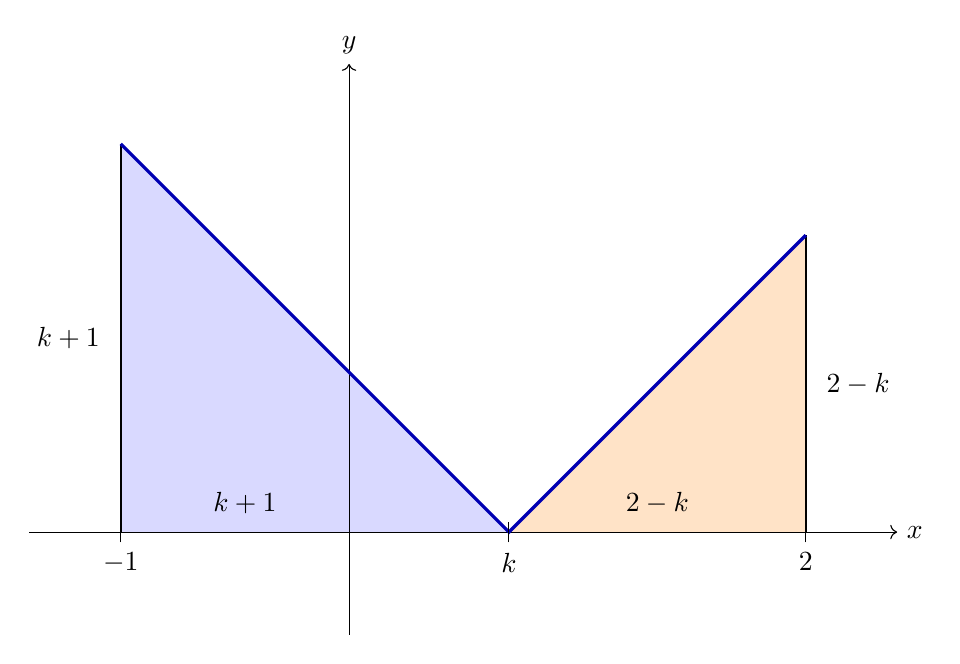
\begin{tikzpicture}[scale=2.9]
\def\kpos{0.7}
\pgfmathsetmacro{\leftheight}{\kpos+1}
\pgfmathsetmacro{\rightheight}{2-\kpos}
\coordinate (L) at (-1,0);
\coordinate (V) at (\kpos,0);
\coordinate (R) at (2,0);
\coordinate (LT) at (-1,\leftheight);
\coordinate (RT) at (2,\rightheight);
\fill[blue!15] (L) -- (LT) -- (V) -- cycle;
\fill[orange!22] (V) -- (RT) -- (R) -- cycle;
\draw[->] (-1.4,0) -- (2.4,0) node[right] {$x$};
\draw[->] (0,-0.45) -- (0,2.05) node[above] {$y$};
\draw[thick,black] (L) -- (LT) (R) -- (RT);
\draw[very thick,blue!70!black] (LT) -- (V) -- (RT);
\foreach \P/\lab in {L/$-1$,V/$k$,R/$2$}{
  \draw[black] ($ (\P)+(0,-0.045) $) -- ($ (\P)+(0,0.045) $);
  \node[below=4pt] at (\P) {\lab};
}
\node[above=3pt] at ($(L)!0.32!(V)$) {$k+1$};
\node[left=4pt] at ($(L)!0.5!(LT)$) {$k+1$};
\node[above=3pt] at ($(V)!0.5!(R)$) {$2-k$};
\node[right=4pt] at ($(R)!0.5!(RT)$) {$2-k$};
\end{tikzpicture}
% end q000134 figure F2
\end{djsSolutionFigure}

The two sloping sides have gradients $-1$ and $1$, so each triangle's height equals its base. This also covers $k=-1$ and $k=2$, when one triangle has zero area.

Using $\text{area of a triangle}=\frac12\times\text{base}\times\text{height}$ gives
\[
A(k)=\frac12(k+1)^2+\frac12(2-k)^2
\]

Expanding,
\[
\begin{aligned}
A(k)&=\frac12(k^2+2k+1)+\frac12(k^2-4k+4)\\[5pt]
&=k^2-k+\frac52
\end{aligned}
\]

Completing the square,
\[
\begin{aligned}
A(k)&=\left(k-\frac12\right)^2-\frac14+\frac52\\[5pt]
&=\left(k-\frac12\right)^2+\frac94
\end{aligned}
\]

The squared term is least when $k=\frac12$, which lies in $-1\le k\le2$. Therefore $A(k)$ is minimised at $k=\frac12$, so the correct option is \textbf{B}.\\[5pt]

\textit{Alternative Solution:}

We can instead split the integral where the expression inside the modulus changes sign. Recall the definition
\[
|x|=\begin{cases}
x,&x\ge0\\[5pt]
-x,&x<0
\end{cases}
\]

For $x\ge k$, we have $x-k\ge0$; for $x<k$, we have $x-k<0$. Hence
\[
|x-k|=\begin{cases}
x-k,&x\ge k\\[5pt]
-x+k,&x<k
\end{cases}
\]

As the graph shows, we need only consider $-1\le k\le2$.

Splitting at $x=k$ gives
\begin{align*}
    A(k)&= \int_{-1}^{2} |x-k|\,\mathrm{d}x  \\[8pt]
        &=\int_{-1}^{k}(-x+k)\,\mathrm{d}x+\int_k^2(x-k)\,\mathrm{d}x
\end{align*}



Evaluating,
\[
\begin{aligned}
A(k)
&=\left[-\frac{x^2}{2}+kx\right]_{-1}^{k}
 +\left[\frac{x^2}{2}-kx\right]_{k}^{2}\\[8pt]
&=\left[\left(-\frac{k^2}{2}+k^2\right)-\left(-\frac12-k\right)\right]
 +\left[(2-2k)-\left(\frac{k^2}{2}-k^2\right)\right]\\[8pt]
&=\left(\frac{k^2}{2}+k+\frac12\right)
 +\left(2-2k+\frac{k^2}{2}\right)\\[8pt]
&=k^2-k+\frac52
\end{aligned}
\]

In completed-square form, this is
\[
A(k)=\left(k-\frac12\right)^2+\frac94
\]

The square is least at $k=\frac12$, which is in the permitted range. The correct option is \textbf{B}.
% end q000134 solution
\end{djsSolution}
\end{enumerate}
\clearpage
\thispagestyle{djssolutions}
\vspace*{8pt}
\djsTopicLine{Proof \& Error Analysis}
\begin{enumerate}[label=\textbf{\arabic*.},leftmargin=*,itemsep=0pt,start=8]
\questionitem[Proof \& Error Analysis]
% begin q000015 stem
Consider the following problem for an integer $n$: \[ \left( \dfrac{1}{3} \right)^{n+2} \ge \left( \dfrac{1}{27} \right)^{n-1} \] A student produces the following argument:

\[ \begin{array}{@{}l l@{}}
\textbf{I:} & \text{$\left( \dfrac{1}{3} \right)^{n+2} \ge \left( \dfrac{1}{27} \right)^{n-1}$} \\[20pt]

\textbf{II:} & \text{$\log_{\frac{1}{3}} \left( \left( \dfrac{1}{3} \right)^{n+2} \right) \ge \log_{\frac{1}{3}} \left( \left( \dfrac{1}{27} \right)^{n-1} \right)$} \\[20pt]

\textbf{III:} & \text{$n+2 \ge (n-1)\log_{\frac{1}{3}} \left( \dfrac{1}{27} \right)$} \\[20pt]

\textbf{IV:} & \text{$n+2 \ge 3(n-1)$} \\[20pt]

\textbf{V:} & \text{$n+2 \ge 3n-3$} \\[20pt]

\textbf{VI:} & \text{$n \le 2$} \\[20pt]
\end{array} \] Which step (if any) in the argument is invalid?
% end q000015 stem

\par\vspace*{12pt}
\begin{tabularx}{\linewidth}{@{}>{\bfseries}l Y@{}}
A &
% begin q000015 choice A
There are no invalid steps; the argument is correct.
% end q000015 choice A
\\[0.8em]
B &
% begin q000015 choice B
Only step \textbf{I} is invalid; the rest are correct.
% end q000015 choice B
\\[0.8em]
C &
% begin q000015 choice C
Only step \textbf{II} is invalid; the rest are correct.
% end q000015 choice C
\\[0.8em]
D &
% begin q000015 choice D
Only step \textbf{III} is invalid; the rest are correct.
% end q000015 choice D
\\[0.8em]
E &
% begin q000015 choice E
Only step \textbf{IV} is invalid; the rest are correct.
% end q000015 choice E
\\[0.8em]
F &
% begin q000015 choice F
Only step \textbf{V} is invalid; the rest are correct.
% end q000015 choice F
\\[0.8em]
G &
% begin q000015 choice G
Only step \textbf{VI} is invalid; the rest are correct.
% end q000015 choice G
\\
\end{tabularx}

\begin{djsSolution}{C}
% begin q000015 solution
The student's final answer claims that every integer $n\le2$ satisfies the original inequality. A useful first check is therefore to choose a simple value from this claimed solution set and substitute it into the original inequality. One value that fails is enough to show that the claimed answer is wrong.

Choose $n=1$: it lies in the student's final range and makes the exponent $n-1$ zero, so the calculation is particularly simple.

In Line I, substitution gives
\[
\left(\frac13\right)^{1+2}=\frac1{27}\geq1=\left(\frac1{27}\right)^{1-1}
\]

which is clearly false.
Thus $n=1$ is a counterexample to the student's claimed answer. This does not make Line I invalid: Line I simply states the inequality we were asked to solve.

We can now use the same value to help locate the error. Each rearrangement should preserve the solution set, so a value rejected by the original inequality should remain rejected at every line. Substituting $n=1$ into successive lines lets us look for the point where it is incorrectly admitted as a solution.

At $n=1$, Line II gives
\[
\log_{\frac13}\left(\left(\frac13\right)^3\right)=3\ge0=\log_{\frac13}\left(\left(\frac1{27}\right)^0\right)
\]

This is true, although Line I was false at the same value of $n$. The step from Line I to Line II has therefore changed the solution set.

The reason is that a logarithm with base between $0$ and $1$ reverses an inequality between positive numbers. For example,
\[
\frac12<1
\]

but
\[
\log_{\frac12}\left(\frac12\right)=1>0=\log_{\frac12}1
\]

Applying $\log_{\frac13}$ to Line I should therefore change $\ge$ to $\le$. Line II is invalid. By elimination, the correct option must therefore be \textbf{C.} \\

The counterexample has located an error, but it does not establish that all the remaining steps are valid. We can check those algebraically, judging each line against the line immediately before it.

Using $\log_b(a^k)=k\log_b a$ and $\log_b b=1$ in Line II gives
\[
n+2\ge(n-1)\log_{\frac13}\left(\frac1{27}\right)
\]

Line III correctly follows from Line II.

Since $\left(\frac13\right)^3=\frac1{27}$, we have
\[
\log_{\frac13}\left(\frac1{27}\right)=3
\]

Substituting this gives
\[
n+2\ge3(n-1)
\]

Line IV is correct.

Expanding gives
\[
n+2\ge3n-3
\]

Line V is correct.

Rearranging gives
\[
5\ge2n
\]

Dividing by $2$ gives
\[
n\le\frac52
\]

As $n$ is an integer, this is equivalent to
\[
n\le2
\]

Line VI is correct. Only Line II is invalid, so the correct option is \textbf{C}.\\[5pt]

\textit{Remark:}

Taking logarithms of both sides of an inequality requires us to consider whether the logarithm is an increasing or decreasing function. Applying an increasing function preserves the order of two inputs; applying a decreasing function reverses it. 

Merely applying the same function to both sides does not guarantee that the inequality sign stays the same.

The sketches illustrate these two possibilities. Both logarithms pass through $(1,0)$, but the graph with base $2$ rises from left to right (is an increasing function), whereas the graph with base $\frac12$ falls (is a decreasing function).

\begin{djsSolutionFigure}
% begin q000015 figure F1
\begin{tikzpicture}
\pgfplotsset{logpanel/.style={
    width=7.6cm, height=6.1cm,
    xmin=0, xmax=4, ymin=-2.6, ymax=2.6,
    axis lines=middle,
    axis line style={black,-{Stealth[length=2mm]}},
    xtick=\empty, ytick=\empty,
    xlabel={$x$},
    ylabel={$y$},
    xlabel style={at={(axis description cs:1,0.5)},anchor=west,xshift=3pt},
    ylabel style={at={(axis description cs:0,1)},anchor=south,yshift=3pt},
    clip=false
}}
\begin{axis}[logpanel,at={(0,0)},anchor=south west]
\addplot[thin,densely dashed,black!45]
    coordinates {(0.5,0) (0.5,-1) (0,-1)};
\addplot[very thick,blue!75!black,domain=0.2:4,samples=160]
    {ln(x)/ln(2)};
\node[blue!75!black,anchor=south] at (axis cs:2,1.5)
    {$y=\log_2 x$};
\addplot[only marks,mark=*,mark size=2pt,blue!75!black]
    coordinates {(0.5,-1) (1,0)};
\draw (axis cs:0.5,-0.06) -- (axis cs:0.5,0.06);
\node[above left,font=\scriptsize,xshift=-2pt,yshift=3pt]
    at (axis cs:1,0) {$x_0=\frac12$};
\node[below,font=\scriptsize,xshift=3pt,yshift=-3pt]
    at (axis cs:1.2,0) {$x_1=1$};
\node[left,font=\scriptsize,xshift=-3pt]
    at (axis cs:0,-1) {$-1$};
\end{axis}
\begin{axis}[logpanel,at={(8.2cm,0)},anchor=south west]
\addplot[thin,densely dashed,black!45]
    coordinates {(0.5,0) (0.5,1) (0,1)};
\addplot[very thick,red!75!black,domain=0.2:4,samples=160]
    {-ln(x)/ln(2)};
\node[red!75!black,anchor=south] at (axis cs:2.7,-1.15)
    {$y=\log_{1/2}x$};
\addplot[only marks,mark=*,mark size=2pt,red!75!black]
    coordinates {(0.5,1) (1,0)};
\draw (axis cs:0.5,-0.06) -- (axis cs:0.5,0.06);
\node[below left,font=\scriptsize,xshift=-2pt,yshift=-3pt]
    at (axis cs:1,0) {$x_0=\frac12$};
\node[above,font=\scriptsize,xshift=3pt,yshift=3pt]
    at (axis cs:1.2,0) {$x_1=1$};
\node[left,font=\scriptsize,xshift=-3pt]
    at (axis cs:0,1) {$1$};
\end{axis}
\end{tikzpicture}
% end q000015 figure F1
\end{djsSolutionFigure}

For positive inputs $x_0<x_1$, the left graph shows how $\log_b x_0<\log_b x_1$ when $b>1$, while the right graph shows how $\log_b x_0>\log_b x_1$ when $0<b<1$. 

The marked inputs $\frac12$ and $1$ make the reversal easy to see: their logarithms to base $2$ are $-1$ and $0$, whereas their logarithms to base $\frac12$ are $1$ and $0$.

Thus
\[\frac12<1\]
and
\[\log_2\frac12<\log_21\]
but
\[\log_{1/2}\frac12>\log_{1/2}1\]

So $\log_2$ preserved the inequality whilst $\log_{1/2}$ reversed it.

Indeed, $\log_2x$ is an \textbf{increasing} function, while $\log_{1/2}x$ is a \textbf{decreasing} function.

More generally, $\log_bx$ is \emph{increasing} for $b>1$ and \emph{decreasing} for $0<b<1$.
% end q000015 solution
\end{djsSolution}
\end{enumerate}
\clearpage
\thispagestyle{djssolutions}
\vspace*{8pt}
\djsTopicLine{Trigonometry}
\begin{enumerate}[label=\textbf{\arabic*.},leftmargin=*,itemsep=0pt,start=9]
\questionitem[Trigonometry]
% begin q000008 stem
The equation \[ 2\cos^2 x - k\sin x = 1 \] has $n$ distinct solutions in the range $0 \le x \le 2\pi$

Consider the following statements: \[ \begin{array}{@{}l l@{}}
\textbf{I:} & \text{$k = 0$ is \textbf{necessary} for $n = 2$} \\[2pt]
\textbf{II:} & \text{$k > 2$ \textbf{only if} $n = 0$}
\end{array} \]
Which of the following statements is/are true?
% end q000008 stem

\par\vspace*{12pt}
\begin{tabularx}{\linewidth}{@{}>{\bfseries}l Y@{}}
A &
% begin q000008 choice A
Neither of them
% end q000008 choice A
\\[0.8em]
B &
% begin q000008 choice B
I only
% end q000008 choice B
\\[0.8em]
C &
% begin q000008 choice C
II only
% end q000008 choice C
\\[0.8em]
D &
% begin q000008 choice D
I and II
% end q000008 choice D
\\
\end{tabularx}

\begin{djsSolution}{A}
% begin q000008 solution
A condition is necessary for $n=2$ if $n=2$ cannot hold without it. Statement I therefore says: if $n=2$, then $k=0$.

Recall that ``A only if B'' means ``if A, then B''. Statement II therefore says: if $k>2$, then $n=0$.

Both statements claim that one condition forces another. To disprove either statement, we need just one example where its first condition holds but its claimed consequence fails.

For I, we would need $n=2$ with $k\ne0$. For II, we would need $k>2$ with $n\ne0$.

These suggest a common target: if we can find $k>2$ giving exactly two solutions, both statements will be false. We do not yet know whether this is possible, so we first rewrite the equation to see how its solutions depend on $k$.
 
To find such a value, first use $\cos^2x=1-\sin^2x$ and set $s=\sin x$. The equation becomes
\[
2(1-s^2)-ks=1
\]

Rearranging and applying the quadratic formula gives
\[
2s^2+ks-1=0
\qquad\Longrightarrow\qquad
s=\frac{-k\pm\sqrt{k^2+8}}4
\]

We need to count only roots satisfying $-1\le s\le1$. A root strictly between $0$ and $1$ gives two angles, so a useful counterexample would have one root in this range and the other below $-1$.

Together, the statements suggest looking for a value with $k>2$ and $n=2$: this would disprove both at once. The simplest integer to test is $k=3$.

When $k=3$ the roots are
\[
s=\frac{-3\pm\sqrt{17}}4
\]

Since $4<\sqrt{17}<5$, the positive root satisfies
\[
\frac14<\frac{-3+\sqrt{17}}4<\frac12
\]

The negative root is outside the range of sine:
\[
\frac{-3-\sqrt{17}}4<\frac{-3-4}{4}=-\frac74<-1
\]

So only the positive root is a possible value of $\sin x$. The sketch shows that this level meets $y=\sin x$ exactly twice for $0\le x\le2\pi$.

\begin{djsSolutionFigure}
% begin q000008 figure F1
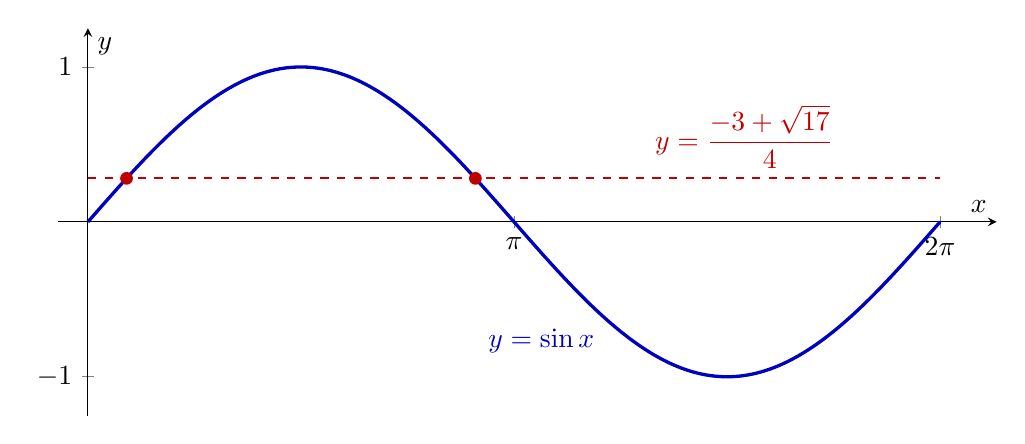
\begin{tikzpicture}
\pgfmathsetmacro{\twopi}{2*pi}
\pgfmathsetmacro{\level}{(-3+sqrt(17))/4}
\pgfmathsetmacro{\firstx}{asin(\level)*pi/180}
\pgfmathsetmacro{\secondx}{pi-\firstx}
\begin{axis}[
    width=13.5cm, height=6.5cm,
    axis lines=middle,
    xlabel={$x$}, ylabel={$y$},
    xmin=-0.22, xmax=6.7,
    ymin=-1.25, ymax=1.25,
    xtick={0,3.141592653589793,6.283185307179586},
    xticklabels={$0$,$\pi$,$2\pi$},
    ytick={-1,1},
    yticklabels={$-1$,$1$},
    clip=true,
]
\addplot[very thick, blue!75!black, domain=0:\twopi, samples=201]
    {sin(deg(x))} node[pos=0.62, below left] {$y=\sin x$};
\addplot[thick, red!75!black, dashed, domain=0:\twopi, samples=2]
    {\level} node[pos=0.77, above] {$y=\dfrac{-3+\sqrt{17}}{4}$};
\fill[red!75!black] (axis cs:\firstx,\level) circle[radius=2.3pt];
\fill[red!75!black] (axis cs:\secondx,\level) circle[radius=2.3pt];
\end{axis}
\end{tikzpicture}
% end q000008 figure F1
\end{djsSolutionFigure}

Neither endpoint is a solution: $\sin0=\sin2\pi=0$, whereas the required sine value is positive. Hence, for $k=3$,
\[
n=2
\]

Statement I is false because $n=2$ but $k\ne0$. Statement II is false because $k>2$ but $n\ne0$. The correct option is \textbf{A}.\\[5pt]

\textit{Alternative Solution:}

We can instead determine the number of solutions for every real value of $k$. As above, putting $s=\sin x$ gives
\[
2s^2+ks-1=0
\]

Its two roots are
\[
s_+=\frac{-k+\sqrt{k^2+8}}4,
\qquad
s_-=\frac{-k-\sqrt{k^2+8}}4
\]

Since $\sqrt{k^2+8}>|k|$, we always have $s_+>0$ and $s_-<0$. We therefore need to check when $s_+\le1$ and when $s_-\ge-1$.

For the positive root,
\[
s_+\le1
\quad\Longleftrightarrow\quad
\sqrt{k^2+8}\le k+4
\]

This requires $k+4\ge0$. Squaring both sides then gives
\[
k^2+8\le(k+4)^2
\quad\Longleftrightarrow\quad
8\le8k+16
\quad\Longleftrightarrow\quad
k\ge-1
\]

This last condition also ensures $k+4\ge0$. Thus the positive root is a permitted sine value exactly when $k\ge-1$, with $s_+=1$ only when $k=-1$.

For the negative root,
\[
s_-\ge-1
\quad\Longleftrightarrow\quad
\sqrt{k^2+8}\le4-k
\]

This requires $4-k\ge0$. Squaring both sides then gives
\[
k^2+8\le(4-k)^2
\quad\Longleftrightarrow\quad
8\le16-8k
\quad\Longleftrightarrow\quad
k\le1
\]

This last condition also ensures $4-k\ge0$. Thus the negative root is a permitted sine value exactly when $k\le1$, with $s_-=-1$ only when $k=1$.

Each nonzero sine value strictly between $-1$ and $1$ gives two solutions for $0\le x\le2\pi$. A sine value of $1$ or $-1$ gives just one. Neither root is zero, so the endpoints $x=0$ and $x=2\pi$ never contribute.

Consequently,
\[
\begin{array}{c|c|c}
\text{Condition on }k & \text{Permitted sine values} & n\\ \hline
k<-1 & \text{One value strictly between }-1\text{ and }0 & 2\\[5pt]
k=-1 & 1\text{ and }-\frac12 & 3\\[5pt]
-1<k<1 & \text{Two values strictly between }-1\text{ and }1 & 4\\[5pt]
k=1 & \frac12\text{ and }-1 & 3\\[5pt]
k>1 & \text{One value strictly between }0\text{ and }1 & 2
\end{array}
\]

Thus $n=2$ whenever $k<-1$ or $k>1$, so $k=0$ is not necessary. Also, every $k>2$ gives $n=2$, not $n=0$. Both statements are false, and the correct option is \textbf{A}.
% end q000008 solution
\end{djsSolution}
\end{enumerate}
\clearpage
\thispagestyle{djssolutions}
\vspace*{8pt}
\djsTopicLine{Inequalities}
\begin{enumerate}[label=\textbf{\arabic*.},leftmargin=*,itemsep=0pt,start=10]
\questionitem[Inequalities]
% begin q000020 stem
A real number $k$ has the property that \[ x^2+kx+1\ge 0 \] for all real $x$ satisfying $x^2-4x+3\le 0$

Which of the following describes the set of all such values of $k$?
% end q000020 stem

\par\vspace*{12pt}
\begin{tabularx}{\linewidth}{@{}>{\bfseries}l Y@{}}
A &
% begin q000020 choice A
$k\ge -2$
% end q000020 choice A
\\[0.8em]
B &
% begin q000020 choice B
$k\ge -\dfrac{10}{3}$
% end q000020 choice B
\\[0.8em]
C &
% begin q000020 choice C
$-2\le k\le 2$
% end q000020 choice C
\\[0.8em]
D &
% begin q000020 choice D
$-4\le k\le 2$
% end q000020 choice D
\\[0.8em]
E &
% begin q000020 choice E
$-4\le k\le 4$
% end q000020 choice E
\\[0.8em]
F &
% begin q000020 choice F
$-6\le k\le -2$
% end q000020 choice F
\\[0.8em]
G &
% begin q000020 choice G
$k\ge 0$
% end q000020 choice G
\\
\end{tabularx}

\begin{djsSolution}{A}
% begin q000020 solution
Factoring the condition on $x$ gives
\[
x^2-4x+3=(x-1)(x-3)\le0
\]

Thus the required inequality must hold for every $x$ satisfying
\[
1\le x\le3
\]

First suppose $x^2+kx+1$ has two distinct real roots. This requires
\[
k^2-4>0
\]

Hence
\[
k<-2\quad\text{or}\quad k>2
\]

Calling the roots $\alpha$ and $\beta$, the quadratic formula gives
\[
\begin{aligned}
\text{smaller root}&=\alpha=\frac{-k-\sqrt{k^2-4}}2\\[8pt]
\text{larger root}&=\beta=\frac{-k+\sqrt{k^2-4}}2
\end{aligned}
\]

An upward-opening quadratic is negative between its two distinct roots. To remain non-negative for every $x$ from $1$ to $3$, both roots must therefore lie at or to the right of $3$, or both must lie at or to the left of $1$.

The schematic sketches illustrate these two arrangements; they show the general shape rather than particular members of the family $y=x^2+kx+1$.

\begin{djsSolutionFigure}
% begin q000020 figure F1
\begin{tikzpicture}[x=1cm,y=1cm]
\colorlet{intervalblue}{blue!75!black}
\colorlet{negativered}{red!65!black}

% The required range lies to the left of both roots.
\begin{scope}
  \draw[->,black] (0,0) -- (6.6,0) node[right] {$x$};
  \draw[thick,black,domain=0.65:5.95,samples=150,variable=\t]
    plot ({\t},{0.24*(\t-4)*(\t-5.6)});
  \draw[very thick,negativered,domain=4:5.6,samples=60,variable=\t]
    plot ({\t},{0.24*(\t-4)*(\t-5.6)});

  \draw[very thick,intervalblue] (1,0) -- (3,0);
  \foreach \p in {1,3} {
    \draw[intervalblue,thick] (\p,-0.07) -- (\p,0.07);
    \node[below=5pt] at (\p,0) {$\p$};
  }

  \draw[black] (4,-0.07) -- (4,0.07);
  \draw[black] (5.6,-0.07) -- (5.6,0.07);
  \node[below=5pt] at (4,0) {$\alpha$};
  \node[below=5pt] at (5.6,0) {$\beta$};
\end{scope}

% The required range lies to the right of both roots.
\begin{scope}[shift={(8cm,0cm)}]
  \draw[->,black] (0,0) -- (6.6,0) node[right] {$x$};
  \draw[thick,black,domain=0.45:5.75,samples=150,variable=\t]
    plot ({\t},{0.24*(\t-0.8)*(\t-2.4)});
  \draw[very thick,negativered,domain=0.8:2.4,samples=60,variable=\t]
    plot ({\t},{0.24*(\t-0.8)*(\t-2.4)});

  \draw[very thick,intervalblue] (3.4,0) -- (5.4,0);
  \draw[intervalblue,thick] (3.4,-0.07) -- (3.4,0.07);
  \draw[intervalblue,thick] (5.4,-0.07) -- (5.4,0.07);
  \node[below=5pt] at (3.4,0) {$1$};
  \node[below=5pt] at (5.4,0) {$3$};

  \draw[black] (0.8,-0.07) -- (0.8,0.07);
  \draw[black] (2.4,-0.07) -- (2.4,0.07);
  \node[below=5pt] at (0.8,0) {$\alpha$};
  \node[below=5pt] at (2.4,0) {$\beta$};
\end{scope}
\end{tikzpicture}
% end q000020 figure F1
\end{djsSolutionFigure}

For the first arrangement, the smaller root $\alpha$ must be at least $3$:
\[
3\le\frac{-k-\sqrt{k^2-4}}2
\]

Rearranging gives
\[
\sqrt{k^2-4}\le-k-6
\]

The square root is non-negative, so the right-hand side must also be non-negative. Hence
\[
k\le-6
\]

We can now square both sides:
\[
\begin{aligned}
k^2-4&\le(-k-6)^2\\[5pt]
k^2-4&\le k^2+12k+36\\[5pt]
-40&\le12k
\end{aligned}
\]

Thus
\[
k\ge-\frac{10}{3}
\]

No $k$ satisfies both $k\le-6$ and $k\ge-\frac{10}{3}$, so this arrangement is impossible. Checking the sign before squaring matters: otherwise we could mistakenly accept values for which $-k-6$ is negative.

For the second arrangement, the larger root $\beta$ must be at most $1$:
\[
1\ge\frac{-k+\sqrt{k^2-4}}2
\]

Rearranging gives
\[
\sqrt{k^2-4}\le k+2
\]

The right-hand side must be non-negative, so
\[
k\ge-2
\]

Squaring both sides gives
\[
\begin{aligned}
k^2-4&\le(k+2)^2\\[5pt]
k^2-4&\le k^2+4k+4\\[5pt]
-8&\le4k
\end{aligned}
\]

This again gives $k\ge-2$. Combining it with the condition for two distinct roots, $k<-2$ or $k>2$, leaves
\[
k>2
\]

We must also consider quadratics without two distinct real roots. When $k^2-4<0$, the upward-opening quadratic is positive everywhere. When $k^2-4=0$, it touches the axis and is non-negative everywhere. These cases together give
\[
-2\le k\le2
\]

Combining this with $k>2$, the complete range is
\[
k\ge-2
\]

The correct option is \textbf{A}.\\[5pt]

\textit{Alternative Solution 1:}

The inequality must hold at every allowed value of $x$, so testing a convenient endpoint can give a necessary condition. At $x=1$,
\[
1^2+k(1)+1=k+2\ge0
\]

Therefore
\[
k\ge-2
\]

Testing one point does not establish that this condition is sufficient. We must also show that every $k\ge-2$ makes the quadratic non-negative for all $x$ from $1$ to $3$.

The boundary value $k=-2$ suggests how to do this, since it gives the perfect square
\[
x^2-2x+1=(x-1)^2
\]

For a general $k\ge-2$, write
\[
x^2+kx+1=(x-1)^2+(k+2)x
\]

Here $(x-1)^2\ge0$, and $(k+2)x\ge0$ because $k+2\ge0$ and $x\ge1$. Hence
\[
x^2+kx+1\ge0
\]

Thus $k\ge-2$ is both necessary and sufficient, so the correct option is \textbf{A}.\\[5pt]

\textit{Remark:} Requiring a non-positive discriminant would ensure that the quadratic is non-negative for every real $x$. That is stronger than the question requires: only values with $1\le x\le3$ matter. In particular, $k>2$ gives two negative roots, so the quadratic can be negative elsewhere while remaining positive throughout the required range.\\[5pt]

\textit{Alternative Solution 2:}

Factoring the restriction gives
\[
(x-1)(x-3)\le0
\]

Hence
\[
1\le x\le3
\]

We can also use the differences between the options to eliminate them. An option is false if it includes a value of $k$ that fails, or excludes a value that works.

Options B, D, E and F all include $k=-3$. This is an easy value to test at the allowed endpoint $x=1$:
\[
1^2+(-3)(1)+1=-1<0
\]

Thus $k=-3$ fails, ruling out all four options.

Of the remaining options A, C and G, only G excludes $k=-2$. But when $k=-2$,
\[
x^2-2x+1=(x-1)^2\ge0
\]

This holds for every real $x$, so $k=-2$ works and G is false.

Finally, A and C differ over whether values greater than $2$ are allowed. Try $k=3$. For every $x$ with $1\le x\le3$, all three terms in $x^2+3x+1$ are positive, so this value works. Option C excludes it and is therefore false.

Only A remains, so the correct option is \textbf{A}.
% end q000020 solution
\end{djsSolution}
\end{enumerate}
\clearpage
\thispagestyle{djssolutions}
\vspace*{8pt}
\djsTopicLine{Functions \& Graphs}
\begin{enumerate}[label=\textbf{\arabic*.},leftmargin=*,itemsep=0pt,start=11]
\questionitem[Functions \& Graphs]
% begin q000133 stem
Consider the curve defined by \[ (|x|-4)^2+(y-1)^2=1 \] How many distinct straight lines passing through the origin are tangents to this curve?
% end q000133 stem

\par\vspace*{12pt}
\begin{tabularx}{\linewidth}{@{}>{\bfseries}l Y@{}}
A &
% begin q000133 choice A
$0$
% end q000133 choice A
\\[0.8em]
B &
% begin q000133 choice B
$1$
% end q000133 choice B
\\[0.8em]
C &
% begin q000133 choice C
$2$
% end q000133 choice C
\\[0.8em]
D &
% begin q000133 choice D
$3$
% end q000133 choice D
\\[0.8em]
E &
% begin q000133 choice E
$4$
% end q000133 choice E
\\[0.8em]
F &
% begin q000133 choice F
$5$
% end q000133 choice F
\\
\end{tabularx}

\begin{djsSolution}{D}
% begin q000133 solution
Split the equation according to the sign of $x$. Recall that
\[
|x|=\begin{cases}
x & x\ge 0\\[5pt]
-x & x\le 0
\end{cases}
\]

For $x\ge0$, the equation becomes
\[
(x-4)^2+(y-1)^2=1
\]

The standard equation $(x-a)^2+(y-b)^2=r^2$ describes a circle with centre $(a,b)$ and radius $r$. This circle has centre $(4,1)$ and radius $1$, so all its points satisfy
\[
3\le x\le5
\]

Thus the restriction $x\ge0$ does not cut off any of the circle.

For $x<0$, substituting $|x|=-x$ gives
\[
(-x-4)^2+(y-1)^2=1
\]

Hence
\[
(x+4)^2+(y-1)^2=1
\]

This is the whole circle with centre $(-4,1)$ and radius $1$: all its points satisfy
\[
-5\le x\le-3
\]

The two circles and their tangent lines through the origin are shown to scale.

\begin{djsSolutionFigure}
% begin q000133 figure F1
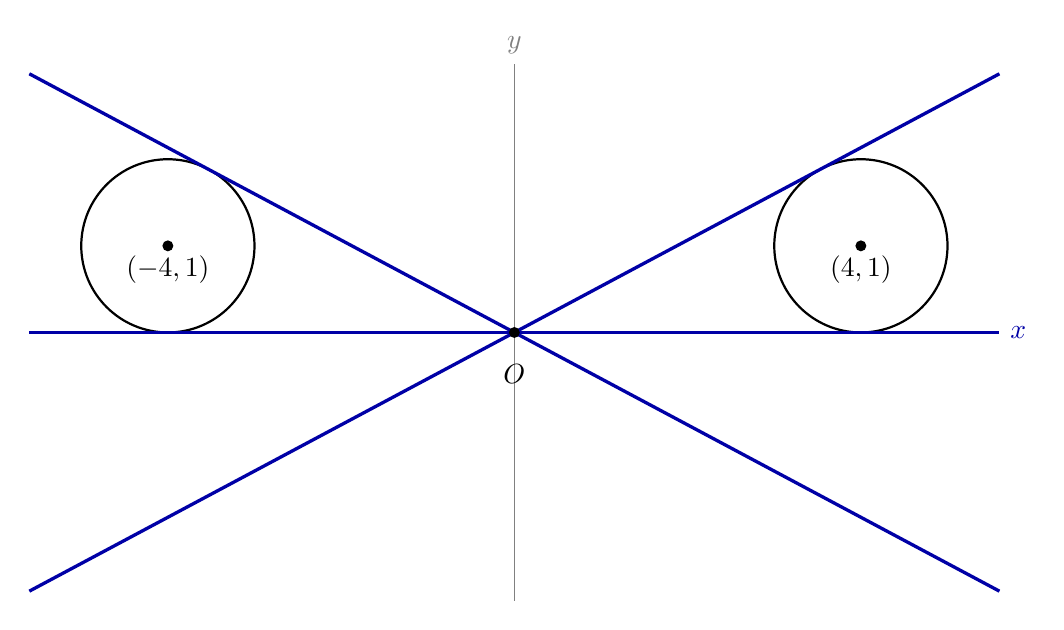
\begin{tikzpicture}[scale=1.1]
\def\xedge{5.6}
\def\yedge{3.1}
\def\radius{1}
\pgfmathsetmacro{\tipy}{8*\xedge/15}
\coordinate (O) at (0,0);
\coordinate (R) at (4,1);
\coordinate (L) at (-4,1);

\draw[thin,gray] (0,-\yedge) -- (0,\yedge) node[above] {$y$};
\draw[thick,black] (L) circle (\radius);
\draw[thick,black] (R) circle (\radius);

\draw[very thick,blue!65!black] (-\xedge,-\tipy) -- (\xedge,\tipy);
\draw[very thick,blue!65!black] (-\xedge,\tipy) -- (\xedge,-\tipy);
\draw[very thick,blue!65!black] (-\xedge,0) -- (\xedge,0) node[right] {$x$};

\fill (O) circle (1.8pt);
\fill (L) circle (1.8pt);
\fill (R) circle (1.8pt);
\node[below=8pt] at (O) {$O$};
\node[below] at (L) {$(-4,1)$};
\node[below] at (R) {$(4,1)$};
\end{tikzpicture}
% end q000133 figure F1
\end{djsSolutionFigure}

The $x$-axis touches both circles, but it is only one distinct line. The sketch shows one further tangent from the origin to each circle; these are reflections in the $y$-axis and are different lines.

Therefore the number of distinct tangent lines is
\[
1+1+1=3
\]

The correct option is \textbf{D}.\\[5pt]

\textit{Alternative Solution:}

For $x\ge0$, the curve is the entire circle $(x-4)^2+(y-1)^2=1$, since its centre is $(4,1)$ and its radius is $1$. A non-vertical line through the origin has equation $y=mx$.

Substituting into the circle equation gives
\[
(x-4)^2+(mx-1)^2=1
\]

Expanding,
\[
x^2-8x+16+m^2x^2-2mx+1=1
\]

Collecting terms,
\[
(1+m^2)x^2-(8+2m)x+16=0
\]

The line is tangent when this quadratic has one repeated root. For a quadratic $ax^2+bx+c=0$, this means its discriminant $b^2-4ac$ is zero.

Here the discriminant is
\[
\begin{aligned}
\Delta&=(8+2m)^2-4(1+m^2)(16)\\[5pt]
&=64+32m+4m^2-64-64m^2\\[5pt]
&=4m(8-15m)
\end{aligned}
\]

Setting $\Delta=0$ gives
\[
4m(8-15m)=0
\]

Therefore the right-hand circle has tangents with slopes
\[
m=0\quad\text{or}\quad m=\frac{8}{15}
\]

Reflection in the $y$-axis changes the slope $m$ to $-m$. The left-hand circle therefore has tangents with slopes
\[
m=0\quad\text{or}\quad m=-\frac{8}{15}
\]

We must also check the vertical line $x=0$, which cannot be written as $y=mx$. Substituting $x=0$ into the original equation gives
\[
16+(y-1)^2=1
\]

This has no real solution, so the vertical line is not a tangent. The three distinct tangent lines have slopes $0$, $\frac{8}{15}$ and $-\frac{8}{15}$, so the correct option is \textbf{D}.
% end q000133 solution
\end{djsSolution}
\end{enumerate}
\clearpage
\thispagestyle{djssolutions}
\vspace*{8pt}
\djsTopicLine{Proof \& Error Analysis}
\begin{enumerate}[label=\textbf{\arabic*.},leftmargin=*,itemsep=0pt,start=12]
\questionitem[Proof \& Error Analysis]
% begin q000647 stem
Let $a$ and $b$ be positive real numbers, neither of which is equal to $1$. 

A student attempts to prove the following claim:
\begin{center} \begin{minipage}{0.82\linewidth} \centering \textbf{Claim:} If  $\log_a b=\log_b a$ then $a=b$ \end{minipage} \end{center}
The student writes the following argument: \[
\begin{array}{@{}ll}
\textbf{Line 1:} & \text{Let } t=\log_a b,\text{ so that }a^t=b \\[4pt]

\textbf{Line 2:} & \text{Since }b\neq1,\text{ we have }t\neq0 \\[4pt]

\textbf{Line 3:} &
\text{Raising both sides of }a^t=b\text{ to the power }\frac1t
\text{ gives }a=b^{1/t} \\[4pt]

\textbf{Line 4:} &
\text{Hence }\log_b a=\frac1t,\text{ so the given condition implies }
t=\frac1t,\text{ and therefore }t^2=1 \\[4pt]

\textbf{Line 5:} &
\text{Since }a^t=b\text{ and both }a\text{ and }b\text{ are positive, we must have }t>0 \\[4pt]

\textbf{Line 6:} & \text{Hence }t=1 \\[4pt]

\textbf{Line 7:} & \text{Therefore }b=a^1=a,\text{ which proves the claim.}
\end{array}
\]

Which line contains the first error?
% end q000647 stem

\par\vspace*{12pt}
\begin{tabularx}{\linewidth}{@{}>{\bfseries}l Y@{}}
A &
% begin q000647 choice A
Line 1
% end q000647 choice A
\\[0.8em]
B &
% begin q000647 choice B
Line 2
% end q000647 choice B
\\[0.8em]
C &
% begin q000647 choice C
Line 3
% end q000647 choice C
\\[0.8em]
D &
% begin q000647 choice D
Line 4
% end q000647 choice D
\\[0.8em]
E &
% begin q000647 choice E
Line 5
% end q000647 choice E
\\[0.8em]
F &
% begin q000647 choice F
Line 6
% end q000647 choice F
\\[0.8em]
G &
% begin q000647 choice G
Line 7
% end q000647 choice G
\\[0.8em]
H &
% begin q000647 choice H
There is no error; the argument is correct.
% end q000647 choice H
\\
\end{tabularx}

\begin{djsSolution}{E}
% begin q000647 solution
We are asked for the first error, so check each step against the information available at that point.

Line 1 uses the definition of a logarithm: $t=\log_a b$ means $a^t=b$. Line 1 is correct.

In Line 2, $a^0=1$, whereas $b\ne1$. Therefore $t\ne0$. Line 2 is correct.

Since $t\ne0$ and both bases are positive, we may raise both sides of $a^t=b$ to the power $1/t$:
\[
(a^t)^{1/t}=b^{1/t}
\]

Using the laws of indices gives
\[
a=b^{1/t}
\]

Line 3 is correct.

By the definition of a logarithm, $b^{1/t}=a$ gives
\[
\log_b a=\frac1t
\]

The given equality of logarithms therefore implies
\[
t=\frac1t
\]

Multiplying by $t\ne0$ gives
\[
t^2=1
\]

Line 4 is correct. At this point, there are two possibilities:
\[
t=1\quad\text{or}\quad t=-1
\]

Line 5 attempts to exclude $t=-1$ using the positivity of $a$ and $b$. But a positive base raised to a negative power still gives a positive number. In particular,
\[
a^{-1}=\frac1a>0
\]

Thus $a^t=b$ with $a,b>0$ does not force $t>0$. The first error is in Line 5, so the correct option is \textbf{E}.

The rejected possibility also gives a counterexample to the claim. Choose $a=2$ and $b=\frac12$. Both satisfy the stated restrictions, and
\[
\begin{aligned}
\log_2\frac12&=-1\\[5pt]
\log_{\frac12}2&=-1
\end{aligned}
\]

The logarithms are equal, but $a\ne b$.\\[5pt]

\textit{Alternative Solution:}

The claim says that equal logarithms force $a=b$. To disprove it, we would need two different allowed values of $a$ and $b$ for which the logarithms are equal.

Reciprocal values are worth trying: if $b=1/a$, then raising either number to the power $-1$ gives the other. Choose $a=2$ and $b=\frac12$. Since
\[
2^{-1}=\frac12
\qquad\text{and}\qquad
\left(\frac12\right)^{-1}=2
\]

we have
\[
\log_2\frac12=\log_{\frac12}2=-1
\]

Thus the hypothesis holds but the conclusion fails. We can now follow this example through the argument to see where the student excludes a possibility that should remain allowed.

Line 1 gives $t=-1$ and $2^{-1}=\frac12$, both of which hold.

Line 2 gives $t\ne0$, which also holds.

In Line 3, raising both sides to the power $1/t=-1$ gives
\[
2=\left(\frac12\right)^{-1}
\]

This is true.

In Line 4,
\[
\log_{\frac12}2=-1=\frac1t
\qquad\text{and}\qquad
t^2=(-1)^2=1
\]

These statements also hold. Line 5, however, claims $t>0$, whereas our example has $t=-1$.

This identifies Line 5 as invalid. Substitution alone does not prove that the earlier lines are valid in general, but their uses of the logarithm definition and index laws are valid, as checked above. The first error is therefore in Line 5, and the correct option is \textbf{E}.\\[5pt]

\textit{Remark:}

The valid steps establish $t^2=1$, so the original condition has two possibilities:
\[
\begin{aligned}
t=1&\quad\Longrightarrow\quad b=a\\[5pt]
t=-1&\quad\Longrightarrow\quad b=\frac1a
\end{aligned}
\]

Both possibilities satisfy the equality of logarithms. The student's mistake is to discard the reciprocal case without justification.

The claim would become true if we additionally required $a>1$ and $b>1$. For a base greater than $1$, a negative power gives a value less than $1$, so $a^t=b>1$ forces $t>0$. Then $t^2=1$ leaves only $t=1$, giving $a=b$.

The distinction is between a positive value and a positive exponent: positivity of $a^t$ alone tells us nothing about the sign of $t$, because every real power of a positive base is positive.
% end q000647 solution
\end{djsSolution}
\end{enumerate}
\clearpage
\thispagestyle{djssolutions}
\vspace*{8pt}
\djsTopicLine{Geometry}
\begin{enumerate}[label=\textbf{\arabic*.},leftmargin=*,itemsep=0pt,start=13]
\questionitem[Geometry]
% begin q000146 stem
Let $C$ be the circle $x^2+y^2=9$

Let $P$ be the point $(a,0)$ where $a>3$

The two tangents from $P$ to $C$ touch the circle at $T_1$ and $T_2$

What is the area of triangle $PT_1T_2$ in terms of $a$?
% end q000146 stem

\par\vspace*{12pt}
\begin{tabularx}{\linewidth}{@{}>{\bfseries}l Y@{}}
A &
% begin q000146 choice A
$3\sqrt{a^2-9}$
% end q000146 choice A
\\[0.8em]
B &
% begin q000146 choice B
$\dfrac{3(a^2-9)^{3/2}}{a^2}$
% end q000146 choice B
\\[0.8em]
C &
% begin q000146 choice C
$\dfrac{9}{a}\sqrt{a^2-9}$
% end q000146 choice C
\\[0.8em]
D &
% begin q000146 choice D
$\dfrac{a}{3}\sqrt{a^2-9}$
% end q000146 choice D
\\[0.8em]
E &
% begin q000146 choice E
$\dfrac{a^2-9}{3}$
% end q000146 choice E
\\[0.8em]
F &
% begin q000146 choice F
$\dfrac{a^2-9}{a}$
% end q000146 choice F
\\[0.8em]
G &
% begin q000146 choice G
$\dfrac{9}{\sqrt{a^2-9}}$
% end q000146 choice G
\\
\end{tabularx}

\begin{djsSolution}{B}
% begin q000146 solution
To find the area of triangle $PT_1T_2$, take $T_1T_2$ as the base and find the perpendicular distance from $P$ to this base.

Let $O$ be the centre of the circle. By symmetry about $OP$, the chord $T_1T_2$ meets $OP$ at its midpoint $H$ and is perpendicular to it. Thus we need the lengths $T_1H$ and $PH$.

The radius to a point of contact is perpendicular to the tangent, so triangle $OT_1P$ is right-angled at $T_1$. Write $\theta=\angle T_1OP$.

\begin{djsSolutionFigure}
% begin q000146 figure F1
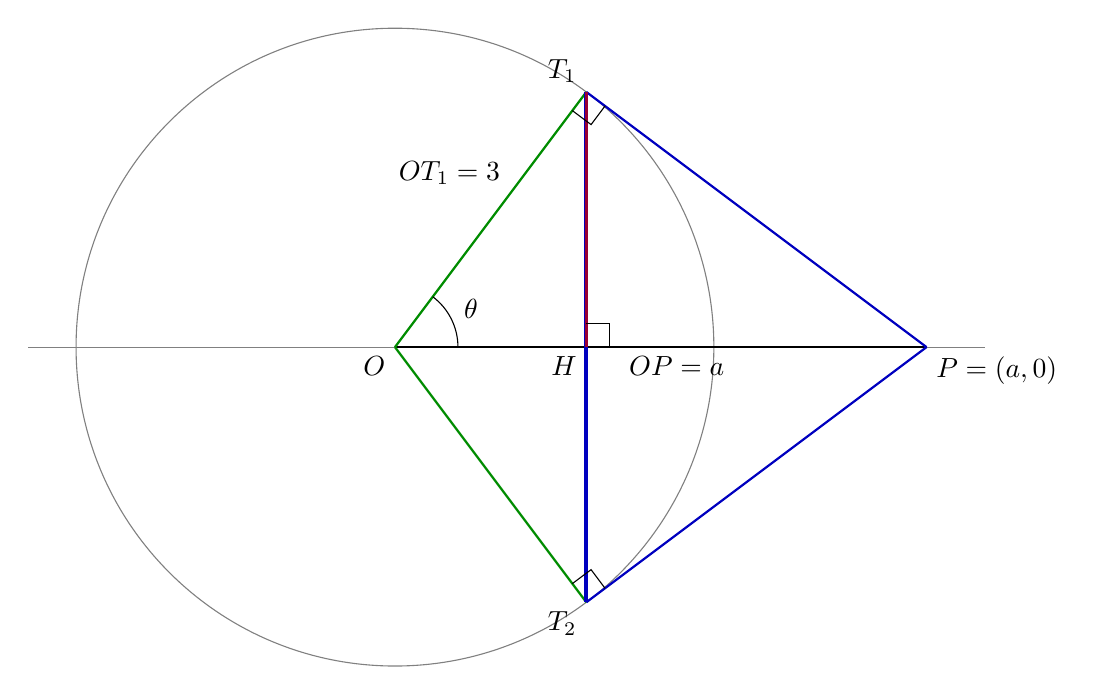
\begin{tikzpicture}[scale=1.35]
\def\aval{5}
\def\radius{3}
\pgfmathsetmacro{\hx}{\radius*\radius/\aval}
\pgfmathsetmacro{\hy}{\radius*sqrt(\aval*\aval-\radius*\radius)/\aval}
\pgfmathsetmacro{\tanglen}{sqrt(\aval*\aval-\radius*\radius)}
\def\marksize{0.22}
\pgfmathsetmacro{\rfrac}{\marksize/\radius}
\pgfmathsetmacro{\tfrac}{\marksize/\tanglen}
\coordinate (O) at (0,0);
\coordinate (P) at (\aval,0);
\coordinate (H) at (\hx,0);
\coordinate (TOne) at (\hx,\hy);
\coordinate (TTwo) at (\hx,-\hy);
\coordinate (Rone) at ($(TOne)!\rfrac!(O)$);
\coordinate (Sone) at ($(TOne)!\tfrac!(P)$);
\coordinate (Rtwo) at ($(TTwo)!\rfrac!(O)$);
\coordinate (Stwo) at ($(TTwo)!\tfrac!(P)$);

\draw[thin,gray] (O) circle (\radius);
\draw[thin,gray] (-3.45,0) -- (5.55,0);
\draw[thick,black] (O) -- (P);
\draw[thick,green!55!black] (O) -- (TOne) (O) -- (TTwo);
\draw[thick,blue!75!black] (P) -- (TOne) (P) -- (TTwo);
\draw[line width=1.5pt,blue!75!black] (TOne) -- (TTwo);
\draw[line width=1.1pt,purple!80!black] (TOne) -- (H);
\draw[thin] (Rone) -- ($(Rone)+(Sone)-(TOne)$) -- (Sone);
\draw[thin] (Rtwo) -- ($(Rtwo)+(Stwo)-(TTwo)$) -- (Stwo);
\draw[thin] ($(H)+(0,\marksize)$) -- ($(H)+(\marksize,\marksize)$) -- ($(H)+(\marksize,0)$);
\pic["$\theta$",draw,angle radius=8mm,angle eccentricity=1.35] {angle=P--O--TOne};

\node[below left] at (O) {$O$};
\node[below right] at (P) {$P=(a,0)$};
\node[above left] at (TOne) {$T_1$};
\node[below left] at (TTwo) {$T_2$};
\node[below left] at (H) {$H$};
\path (O) -- node[pos=0.60,above left] {$OT_1=3$} (TOne);
\path (O) -- node[pos=0.53,below] {$OP=a$} (P);
\end{tikzpicture}
% end q000146 figure F1
\end{djsSolutionFigure}

The circle has radius $3$, so $OT_1=3$, while $OP=a$. Applying Pythagoras in triangle $OT_1P$ gives
\[
PT_1=\sqrt{OP^2-OT_1^2}=\sqrt{a^2-9}
\]

In the same triangle,
\[
\begin{aligned}
\cos\theta&=\frac{OT_1}{OP}=\frac3a\\[8pt]
\sin\theta&=\frac{PT_1}{OP}=\frac{\sqrt{a^2-9}}a
\end{aligned}
\]

These ratios let us find the sides of the smaller right-angled triangle $OT_1H$, which shares the angle $\theta$ at $O$ and has hypotenuse $OT_1=3$:
\[
\begin{aligned}
OH&=OT_1\cos\theta
=3\left(\frac3a\right)
=\frac9a\\[8pt]
T_1H&=OT_1\sin\theta
=3\left(\frac{\sqrt{a^2-9}}a\right)
=\frac{3\sqrt{a^2-9}}a
\end{aligned}
\]

Since $H$ is the midpoint of $T_1T_2$, the base is
\[
T_1T_2=2T_1H=\frac{6\sqrt{a^2-9}}a
\]

The perpendicular height is $PH$. Subtracting $OH$ from $OP$ gives
\[
PH=a-\frac9a=\frac{a^2-9}a
\]

\begin{djsSolutionFigure}
% begin q000146 figure F2
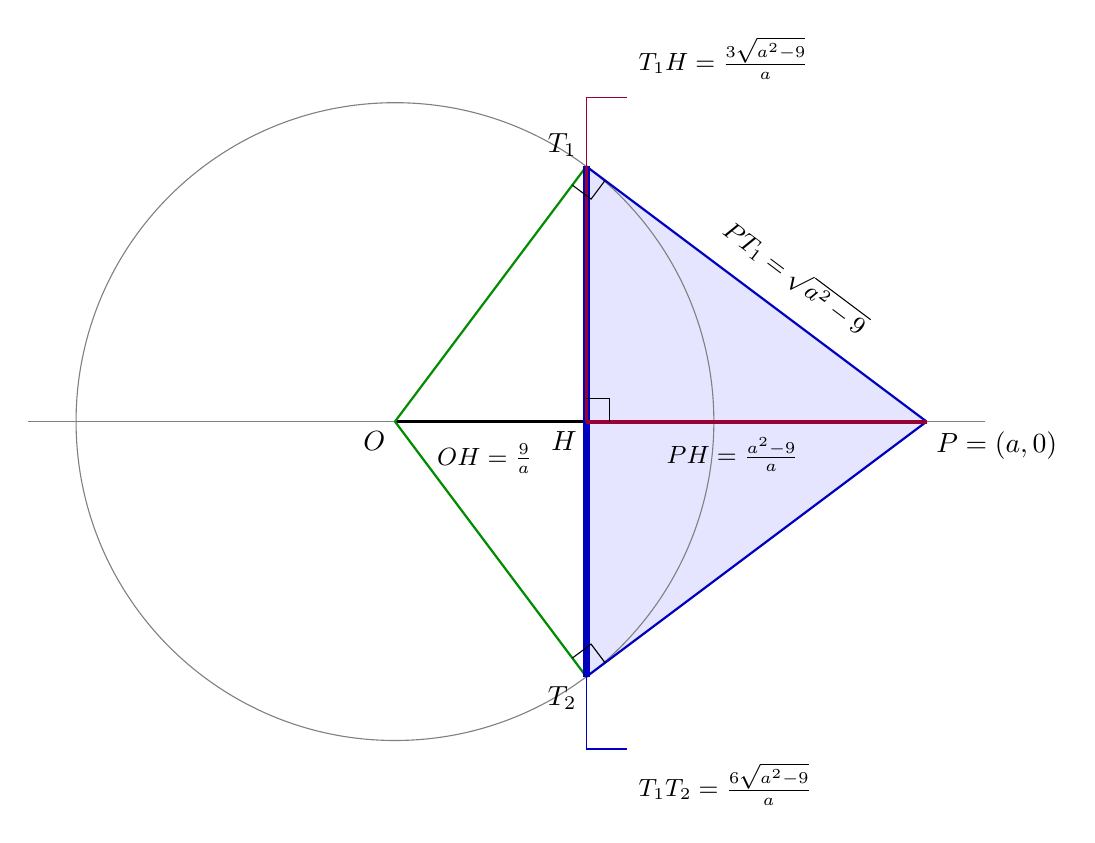
\begin{tikzpicture}[scale=1.35]
\def\aval{5}
\def\radius{3}
\pgfmathsetmacro{\hx}{\radius*\radius/\aval}
\pgfmathsetmacro{\hy}{\radius*sqrt(\aval*\aval-\radius*\radius)/\aval}
\pgfmathsetmacro{\tanglen}{sqrt(\aval*\aval-\radius*\radius)}
\def\marksize{0.22}
\pgfmathsetmacro{\rfrac}{\marksize/\radius}
\pgfmathsetmacro{\tfrac}{\marksize/\tanglen}
\coordinate (O) at (0,0);
\coordinate (P) at (\aval,0);
\coordinate (H) at (\hx,0);
\coordinate (TOne) at (\hx,\hy);
\coordinate (TTwo) at (\hx,-\hy);
\coordinate (Rone) at ($(TOne)!\rfrac!(O)$);
\coordinate (Sone) at ($(TOne)!\tfrac!(P)$);
\coordinate (Rtwo) at ($(TTwo)!\rfrac!(O)$);
\coordinate (Stwo) at ($(TTwo)!\tfrac!(P)$);

\fill[blue!10] (P) -- (TOne) -- (TTwo) -- cycle;
\draw[thin,gray] (O) circle (\radius);
\draw[thin,gray] (-3.45,0) -- (5.55,0);
\draw[thick,black] (O) -- (P);
\draw[thick,green!55!black] (O) -- (TOne) (O) -- (TTwo);
\draw[thick,blue!75!black] (P) -- (TOne) (P) -- (TTwo);
\draw[line width=2.3pt,blue!75!black] (TOne) -- (TTwo);
\draw[line width=1.1pt,purple!80!black] (TOne) -- (H);
\draw[line width=1.4pt,purple!80!black] (H) -- (P);
\draw[thin] (Rone) -- ($(Rone)+(Sone)-(TOne)$) -- (Sone);
\draw[thin] (Rtwo) -- ($(Rtwo)+(Stwo)-(TTwo)$) -- (Stwo);
\draw[thin] ($(H)+(0,\marksize)$) -- ($(H)+(\marksize,\marksize)$) -- ($(H)+(\marksize,0)$);

\node[below left] at (O) {$O$};
\node[below right] at (P) {$P=(a,0)$};
\node[above left] at (TOne) {$T_1$};
\node[below left] at (TTwo) {$T_2$};
\node[below left] at (H) {$H$};
\node[font=\small] at ($(O)!0.47!(H)+(0,-0.35)$) {$OH=\frac{9}{a}$};
\node[font=\small] at ($(H)!0.43!(P)+(0,-0.31)$) {$PH=\frac{a^2-9}{a}$};
\path (TOne) -- node[pos=0.55,above=5pt,sloped,font=\small] {$PT_1=\sqrt{a^2-9}$} (P);
\draw[thin,purple!80!black] (TOne) -- ($(TOne)+(0,0.65)$) -- ($(TOne)+(0.38,0.65)$);
\node[anchor=west,font=\small] at ($(TOne)+(0.40,1.02)$) {$T_1H=\frac{3\sqrt{a^2-9}}{a}$};
\draw[thin,blue!75!black] (TTwo) -- ($(TTwo)+(0,-0.68)$) -- ($(TTwo)+(0.38,-0.68)$);
\node[anchor=west,font=\small] at ($(TTwo)+(0.40,-1.01)$) {$T_1T_2=\frac{6\sqrt{a^2-9}}{a}$};
\end{tikzpicture}
% end q000146 figure F2
\end{djsSolutionFigure}

Using $\text{area}=\frac12\times\text{base}\times\text{perpendicular height}$ gives
\[
\begin{aligned}
\text{Area of }PT_1T_2
&=\frac12\times\frac{6\sqrt{a^2-9}}a\times\frac{a^2-9}a\\[8pt]
&=\frac{3(a^2-9)\sqrt{a^2-9}}{a^2}\\[8pt]
&=\frac{3(a^2-9)^{3/2}}{a^2}
\end{aligned}
\]

The correct option is \textbf{B}.
% end q000146 solution
\end{djsSolution}
\end{enumerate}
\clearpage
\thispagestyle{djssolutions}
\vspace*{8pt}
\djsTopicLine{Functions \& Graphs}
\begin{enumerate}[label=\textbf{\arabic*.},leftmargin=*,itemsep=0pt,start=14]
\questionitem[Functions \& Graphs]
% begin q000038 stem
Let $f(x)=|x-1|$ and $g(x)=|x+1|$

Define \[ h(x)=f\bigl(g(x)\bigr) \] How many integers $x$ satisfy $h(x)<1$?
% end q000038 stem

\par\vspace*{12pt}
\begin{tabularx}{\linewidth}{@{}>{\bfseries}l Y@{}}
A &
% begin q000038 choice A
$0$
% end q000038 choice A
\\[0.8em]
B &
% begin q000038 choice B
$1$
% end q000038 choice B
\\[0.8em]
C &
% begin q000038 choice C
$2$
% end q000038 choice C
\\[0.8em]
D &
% begin q000038 choice D
$3$
% end q000038 choice D
\\[0.8em]
E &
% begin q000038 choice E
$4$
% end q000038 choice E
\\[0.8em]
F &
% begin q000038 choice F
$5$
% end q000038 choice F
\\
\end{tabularx}

\begin{djsSolution}{C}
% begin q000038 solution
Substitute $g(x)=|x+1|$ into $f$:
\[
h(x)=f(g(x))=\bigl||x+1|-1\bigr|
\]

For integer $x$, adding or subtracting $1$ and taking an absolute value all give integers. Thus $h(x)$ is an integer; the outer absolute value also gives $h(x)\ge0$.

The only integer that is non-negative and less than $1$ is $0$, so we need
\[
h(x)=0
\]

Therefore
\[
\bigl||x+1|-1\bigr|=0
\]

An absolute value is zero only when the expression inside it is zero. Hence
\[
|x+1|-1=0
\]

Adding $1$ gives
\[
|x+1|=1
\]

Therefore
\[
x+1=1\quad\text{or}\quad x+1=-1
\]

Subtracting $1$ gives
\[
x=0\quad\text{or}\quad x=-2
\]

There are two such integers, so the correct option is \textbf{C}.\\[5pt]

\textit{Alternative Solution:}

We can instead solve the inequality for real $x$ and then count the integers that satisfy it.

For any real expression $v$, $|v|<1$ means $-1<v<1$. Thus
\[
\bigl||x+1|-1\bigr|<1
\quad\Longleftrightarrow\quad
-1<|x+1|-1<1
\]

Adding $1$ throughout gives
\[
0<|x+1|<2
\]

The sketch of $y=|x+1|$ shows where the graph lies strictly above $y=0$ and strictly below $y=2$. It meets $y=2$ at $x=-3$ and $x=1$, and meets $y=0$ at its vertex, where $x=-1$.

\begin{djsSolutionFigure}
% begin q000038 figure F1
\begin{tikzpicture}[x=2cm,y=1.6cm]
\draw[->] (-3.8,0) -- (1.9,0) node[right] {$x$};
\draw[->] (0,-0.45) -- (0,3.1) node[above] {$y$};

\draw[thick,black!55] (-3.6,2.6) -- (-1,0) -- (1.6,2.6);
\draw[very thick,blue!75!black] (-3,2) -- (-1,0) -- (1,2);
\draw[thick,dashed,orange!85!black] (-3.6,2) -- (1.65,2)
  node[right] {$y=2$};

\draw[thin,densely dashed,black!50] (-3,0) -- (-3,2);
\draw[thin,densely dashed,black!50] (1,0) -- (1,2);

\foreach \p in {-3,-1,1} {
  \draw (\p,-0.06) -- (\p,0.06);
  \node[below=5pt] at (\p,0) {$\p$};
}
\node[below left=3pt] at (0,0) {$0$};
\node[above right,blue!75!black] at (-2.4,1.35) {$y=|x+1|$};

\foreach \p/\q in {-3/2,-1/0,1/2} {
  \draw[blue!75!black,line width=1pt,fill=white]
    (\p,\q) circle[radius=2.5pt];
}
\end{tikzpicture}
% end q000038 figure F1
\end{djsSolutionFigure}

The upper bound $|x+1|<2$ therefore gives
\[
-3<x<1
\]

The lower bound $0<|x+1|$ excludes the vertex $x=-1$. Both inequalities are strict, so the three points marked with open circles are excluded.

The integers satisfying $-3<x<1$ are $-2$, $-1$ and $0$. Removing $-1$ leaves
\[
x=-2\quad\text{or}\quad x=0
\]

There are two, so the correct option is \textbf{C}.
% end q000038 solution
\end{djsSolution}
\end{enumerate}
\clearpage
\thispagestyle{djssolutions}
\vspace*{8pt}
\djsTopicLine{Geometry}
\begin{enumerate}[label=\textbf{\arabic*.},leftmargin=*,itemsep=0pt,start=15]
\questionitem[Geometry]
% begin q000579 stem
A cuboid has edge lengths $a$, $b$ and $c$. The diagonals of its three different rectangular faces have lengths $5\text{ cm}$, $\sqrt{153}\text{ cm}$ and $4\sqrt{10}\text{ cm}$.

What is the volume of the cuboid?
% end q000579 stem

\par\vspace*{12pt}
\begin{tabularx}{\linewidth}{@{}>{\bfseries}l Y@{}}
A &
% begin q000579 choice A
$60\text{ cm}^3$
% end q000579 choice A
\\[0.8em]
B &
% begin q000579 choice B
$144\text{ cm}^3$
% end q000579 choice B
\\[0.8em]
C &
% begin q000579 choice C
$156\text{ cm}^3$
% end q000579 choice C
\\[0.8em]
D &
% begin q000579 choice D
$180\text{ cm}^3$
% end q000579 choice D
\\[0.8em]
E &
% begin q000579 choice E
$240\text{ cm}^3$
% end q000579 choice E
\\[0.8em]
F &
% begin q000579 choice F
$624\text{ cm}^3$
% end q000579 choice F
\\
\end{tabularx}

\begin{djsSolution}{B}
% begin q000579 solution
Each given diagonal belongs to a rectangular face, so Pythagoras relates its length to two edge lengths. Label the front face with sides $a$ and $b$, the top face with sides $b$ and $c$, and the side face with sides $a$ and $c$, as shown.

\begin{djsSolutionFigure}
% begin q000579 figure F1
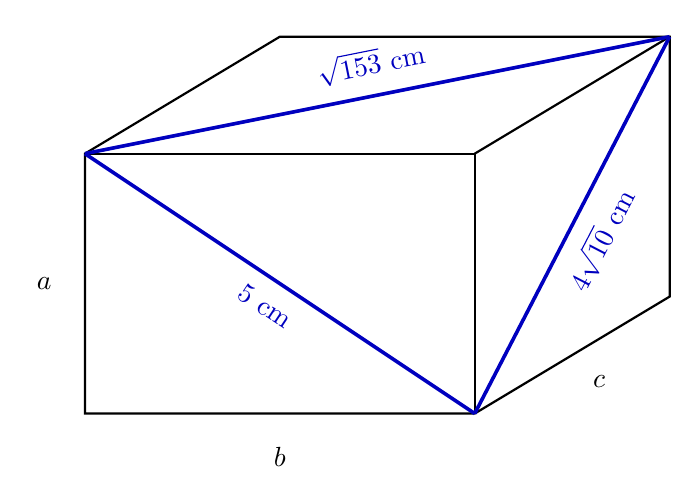
\begin{tikzpicture}[scale=1.65]
\coordinate (A) at (0,0);
\coordinate (B) at (3,0);
\coordinate (C) at (3,2);
\coordinate (D) at (0,2);
\coordinate (F) at (4.5,0.9);
\coordinate (G) at (4.5,2.9);
\coordinate (H) at (1.5,2.9);

% Visible cuboid edges; hidden edges are omitted.
\draw[thick,black] (A)--(B)--(F)--(G)--(H)--(D)--cycle;
\draw[thick,black] (B)--(C)--(D);
\draw[thick,black] (C)--(G);

% One highlighted diagonal on each rectangular face.
\draw[blue!75!black,line width=1.3pt] (D)--(B);
\draw[blue!75!black,line width=1.3pt] (B)--(G);
\draw[blue!75!black,line width=1.3pt] (D)--(G);

% Edge lengths.
\path (A)--(D) node[midway,left=3mm] {$a$};
\path (A)--(B) node[midway,below=3mm] {$b$};
\path (B)--(F) node[midway,below right=2mm] {$c$};

% Face-diagonal lengths.
\path (D)--(B)
  node[midway,sloped,below=3pt,text=blue!75!black]
  {$5\text{ cm}$};
\path (B)--(G)
  node[midway,sloped,below=3pt,text=blue!75!black]
  {$4\sqrt{10}\text{ cm}$};
\path (D)--(G)
  node[midway,sloped,above=3pt,text=blue!75!black]
  {$\sqrt{153}\text{ cm}$};
\end{tikzpicture}
% end q000579 figure F1
\end{djsSolutionFigure}

Applying Pythagoras to the three faces gives
\[
\begin{aligned}
a^2+b^2&=25 &&\text{(1)}\\[5pt]
b^2+c^2&=153 &&\text{(2)}\\[5pt]
a^2+c^2&=160 &&\text{(3)}
\end{aligned}
\]

Subtracting equation (2) from equation (3) eliminates $c^2$:
\[
a^2-b^2=7
\]

Adding this to equation (1) eliminates $b^2$:
\[
2a^2=32
\]

Hence
\[
a^2=16
\]

Substituting into equation (1), then equation (2), gives
\[
\begin{aligned}
b^2&=25-16=9\\[5pt]
c^2&=153-9=144
\end{aligned}
\]

Edge lengths are positive, so
\[
a=4,\qquad b=3,\qquad c=12
\]

The volume is
\[
abc=4\times3\times12=144\text{ cm}^3
\]

The correct option is \textbf{B}.
% end q000579 solution
\end{djsSolution}
\end{enumerate}
\clearpage
\thispagestyle{djssolutions}
\vspace*{8pt}
\djsTopicLine{Proof \& Error Analysis}
\begin{enumerate}[label=\textbf{\arabic*.},leftmargin=*,itemsep=0pt,start=16]
\questionitem[Proof \& Error Analysis]
% begin q000677 stem
A student attempts to prove the following claim.

\begin{center}
\begin{minipage}{0.82\linewidth}
\centering
\textbf{Claim:} For every real number $k$ with $k>\frac{2}{3}$ the equation \\ \qquad\qquad$x^3-3k^2x+k=0$ has three distinct real solutions.
\end{minipage}
\end{center}

The student produces the following argument:\\
\[
\begin{array}{@{}rl@{}}
\textbf{L1} & \text{Let } f(x)=x^3-3k^2x+k \text{, so } f'(x)=3x^2-3k^2 \text{, and } f'(x)=0 \text{ exactly when } \\ & x=-k \text{ or } x=k \text{,} 
  \text{and these two values are different because } k\neq0 \\[5pt]
\textbf{L2} & \text{We have } f'(x)>0 \text{ for } x<-k \text{ and for } x>k \text{, and } f'(x)<0 \text{ for } -k<x<k \\ & \text{so } f \text{ has a local maximum at } x=-k \text{ and a local minimum at } x=k \\[5pt]
\textbf{L3} & \text{The local maximum value is } f(-k)=2k^3+k \text{, which is positive because } k>0 \\[5pt]
\textbf{L4} & \text{The local minimum value is }
f(k)=k-2k^3<0\\[5pt]
\textbf{L5} & \text{A cubic with positive } x^3 \text{ coefficient whose local maximum value is positive and} \\
 & \text{whose local minimum value is negative meets the } x \text{-axis at three different points, so the} \\
 & \text{equation has three distinct real solutions}\\[5pt]
\end{array}
\]

Which one of the following statements about this argument is correct?
% end q000677 stem

\par\vspace*{12pt}
\begin{tabularx}{\linewidth}{@{}>{\bfseries}l Y@{}}
A &
% begin q000677 choice A
The first error is on line L1
% end q000677 choice A
\\[0.8em]
B &
% begin q000677 choice B
The first error is on line L2
% end q000677 choice B
\\[0.8em]
C &
% begin q000677 choice C
The first error is on line L3
% end q000677 choice C
\\[0.8em]
D &
% begin q000677 choice D
The first error is on line L4
% end q000677 choice D
\\[0.8em]
E &
% begin q000677 choice E
The first error is on line L5
% end q000677 choice E
\\[0.8em]
F &
% begin q000677 choice F
There is no error, and the claim is true.
% end q000677 choice F
\\[0.8em]
G &
% begin q000677 choice G
There is no error in any line, but the claim is false.
% end q000677 choice G
\\
\end{tabularx}

\begin{djsSolution}{D}
% begin q000677 solution
We need to identify the first unjustified step, so check the lines in order. There is no need to solve the cubic.

In L1, differentiating gives
\[
f'(x)=3x^2-3k^2=3(x-k)(x+k)
\]

Since $k>\frac23>0$, the derivative is zero at the two distinct values $x=-k$ and $x=k$. L1 is correct.

For L2, the factors $x-k$ and $x+k$ have the same sign when $x<-k$ or $x>k$, and opposite signs when $-k<x<k$. The graph therefore rises, then falls, then rises again. This gives a local maximum at $x=-k$ and a local minimum at $x=k$. L2 is correct.

In L3, substituting $x=-k$ gives
\[
f(-k)=(-k)^3-3k^2(-k)+k=2k^3+k>0
\]

Both terms are positive because $k>0$. L3 is correct.

In L4, the calculation of the minimum value is correct:
\[
\begin{aligned}
f(k)&=k^3-3k^3+k\\[5pt]
&=k-2k^3\\[5pt]
&=k(1-2k^2)
\end{aligned}
\]

However, its sign needs checking. Since $k>0$, this expression is negative precisely when
\[
1-2k^2<0
\]

Rearranging gives
\[
k^2>\frac12
\]

Since $k>0$, this requires
\[
k>\frac1{\sqrt2}
\]

The question only gives $k>\frac23$, which does not guarantee this stronger condition. To compare the two bounds, square them:
\[
\left(\frac23\right)^2=\frac49<\frac12=\left(\frac1{\sqrt2}\right)^2
\]

Both bounds are positive, so $\frac23<\frac1{\sqrt2}$. There are therefore allowed values of $k$ for which the local minimum is not negative.

For a concrete example, choose $k=\frac7{10}$, which lies above $\frac23$ but below $\frac1{\sqrt2}$. Substituting gives
\[
\begin{aligned}
f\left(\frac7{10}\right)
&=\frac7{10}-2\left(\frac7{10}\right)^3\\[5pt]
&=\frac{700-686}{1000}\\[5pt]
&=\frac7{500}>0
\end{aligned}
\]

This contradicts the negative sign asserted in L4, so L4 is the first error.

The graphical reasoning in L5 is valid: if the local maximum is above the $x$-axis and the local minimum is below it, the cubic crosses the axis once before the maximum, once between the turning points and once after the minimum. The error is that L4 claims the minimum is below the axis for every allowed $k$.

The correct option is \textbf{D}.
% end q000677 solution
\end{djsSolution}
\end{enumerate}
\clearpage
\thispagestyle{djssolutions}
\vspace*{8pt}
\djsTopicLine{Polynomials}
\begin{enumerate}[label=\textbf{\arabic*.},leftmargin=*,itemsep=0pt,start=17]
\questionitem[Polynomials]
% begin q000074 stem
Consider the statement:

\[ \begin{array}{c}
\text{For all real numbers $x$, \textbf{if} $x^2+px+1\le 0$ \textbf{then} $x\le 2$}
\end{array} \tag{$\ast$} \]

What is the complete set of real values of $p$ for which ($\ast$) is true?
% end q000074 stem

\par\vspace*{12pt}
\begin{tabularx}{\linewidth}{@{}>{\bfseries}l Y@{}}
A &
% begin q000074 choice A
no real values of $p$
% end q000074 choice A
\\[0.8em]
B &
% begin q000074 choice B
all real values of $p$
% end q000074 choice B
\\[0.8em]
C &
% begin q000074 choice C
$p\ge 0$
% end q000074 choice C
\\[0.8em]
D &
% begin q000074 choice D
$p<0$
% end q000074 choice D
\\[0.8em]
E &
% begin q000074 choice E
$p\ge -\dfrac{5}{2}$
% end q000074 choice E
\\[0.8em]
F &
% begin q000074 choice F
$p<-4$ \textbf{or} $p>0$
% end q000074 choice F
\\
\end{tabularx}

\begin{djsSolution}{E}
% begin q000074 solution
The statement fails only if some $x>2$ satisfies $x^2+px+1\le0$. We therefore need
\[
x^2+px+1>0\qquad\text{for every }x>2
\]

This is the \textbf{contrapositive} of the original statement: ``if $A$ then $B$'' is equivalent to ``if not $B$ then not $A$''.

We can check this by considering the roots of the quadratic. Its discriminant is $p^2-4$. If
\[
p^2-4<0
\]

then
\[
-2<p<2
\]

For these values of $p$, the graph has no roots and opens upwards, so the quadratic is positive for every real $x$. All these values work.

For the remaining values, $p\le-2$ or $p\ge2$, the quadratic has real roots, possibly equal. It is zero or negative between the roots, including the roots themselves. Thus the original statement holds exactly when the larger root is at most $2$. Equality is allowed because $x=2$ satisfies the required conclusion.

By the quadratic formula, we therefore require
\[
\frac{-p+\sqrt{p^2-4}}2\le2
\]

If $p\ge2$, then $\sqrt{p^2-4}<p$, so
\[
\frac{-p+\sqrt{p^2-4}}2<0<2
\]

Thus every $p\ge2$ works.

Now suppose $p\le-2$. Rearranging the root inequality gives
\[
\sqrt{p^2-4}\le p+4
\]

The left-hand side is non-negative, so the right-hand side must also be non-negative:
\[
p\ge-4
\]

With this restriction, we can square both sides without changing the condition:
\[
\begin{aligned}
p^2-4&\le(p+4)^2\\[5pt]
p^2-4&\le p^2+8p+16\\[5pt]
-20&\le8p
\end{aligned}
\]

Hence
\[
p\ge-\frac52
\]

This also satisfies the sign restriction $p\ge-4$. Within the case $p\le-2$, the permitted values are therefore
\[
-\frac52\le p\le-2
\]

Combining this with $-2<p<2$ and $p\ge2$ gives the complete range
\[
p\ge-\frac52
\]

The correct option is \textbf{E}.\\[5pt]

\textit{Alternative Solution:}

We can also distinguish the options by testing convenient values of $p$. To rule out an option, we can either find a value it excludes that works, or a value it includes that fails.

Start with $p=0$. Then $x^2+1>0$ for every real $x$, so no $x$ satisfies the premise $x^2+1\le0$. There can therefore be no counterexample to the statement, and $p=0$ works. This rules out A, D and F, which all exclude $p=0$.

Of the remaining options, try $p=-2$, since it gives a familiar square:
\[
x^2-2x+1=(x-1)^2
\]

This is at most zero only when $x=1$. Since $1\le2$, the statement holds for $p=-2$. This rules out C.

Only B and E remain. They disagree about values below $-\frac52$, so try $p=-3$. To show that this value fails, we need an $x>2$ for which $x^2-3x+1\le0$.

At $x=2$,
\[
2^2-3(2)+1=-1
\]

This suggests trying a nearby value greater than $2$: $x=2$ itself cannot be a counterexample because it satisfies $x\le2$. Taking $x=\frac52$ gives
\[
\begin{aligned}
\left(\frac52\right)^2-3\left(\frac52\right)+1
&=\frac{25}{4}-\frac{30}{4}+\frac44\\[5pt]
&=-\frac14\le0
\end{aligned}
\]

Here the premise holds but the conclusion fails, since $\frac52>2$. Thus $p=-3$ does not work, ruling out B.

Only E remains, so the correct option is \textbf{E}. The first solution establishes the complete range directly; this method identifies it by eliminating the other choices.
% end q000074 solution
\end{djsSolution}
\end{enumerate}
\clearpage
\thispagestyle{djssolutions}
\vspace*{8pt}
\djsTopicLine{Sequences \& Series}
\begin{enumerate}[label=\textbf{\arabic*.},leftmargin=*,itemsep=0pt,start=18]
\questionitem[Sequences \& Series]
% begin q000053 stem
A sequence $x_n$ is defined by $x_1=1$ and \[x_{n+1}=\frac{1}{3}x_n+2\] for $n\ge 1$.

Let $S$ be the sum to infinity of the series \[ \sum_{n=1}^{\infty} \left(x_{n+1}-x_n\right) \] What is the value of $S$?
% end q000053 stem

\par\vspace*{12pt}
\begin{tabularx}{\linewidth}{@{}>{\bfseries}l Y@{}}
A &
% begin q000053 choice A
$-\,\frac{3}{2}$
% end q000053 choice A
\\[0.8em]
B &
% begin q000053 choice B
$-1$
% end q000053 choice B
\\[0.8em]
C &
% begin q000053 choice C
$2$
% end q000053 choice C
\\[0.8em]
D &
% begin q000053 choice D
$\frac{9}{2}$
% end q000053 choice D
\\[0.8em]
E &
% begin q000053 choice E
The series does not converge.
% end q000053 choice E
\\
\end{tabularx}

\begin{djsSolution}{C}
% begin q000053 solution
Within the TMUA specification, an infinite series to be evaluated is expected to be geometric, perhaps after some rearrangement. This suggests looking for a common ratio between the terms being added.

Here those terms are the differences $x_{n+1}-x_n$. Subtracting two versions of the recurrence will cancel the constant $2$, allowing us to compare consecutive differences.

Write
\[
d_n=x_{n+1}-x_n
\]

The recurrence gives
\[
x_2=\frac13(1)+2=\frac73
\]

Thus the first term of the series is
\[
d_1=x_2-x_1=\frac73-1=\frac43
\]

For consecutive differences,
\[
\begin{aligned}
d_{n+1}&=x_{n+2}-x_{n+1}\\[5pt]
&=\left(\frac13x_{n+1}+2\right)-\left(\frac13x_n+2\right)\\[5pt]
&=\frac13(x_{n+1}-x_n)\\[5pt]
&=\frac13d_n
\end{aligned}
\]

The differences therefore form a geometric sequence with first term $\frac43$ and common ratio $\frac13$. Hence
\[
S=\frac43+\frac49+\frac4{27}+\cdots
\]

For a geometric series with first term $a$ and common ratio $r$, the sum to infinity is $\frac{a}{1-r}$ when $|r|<1$. Here $r=\frac13$, so
\[
S=\frac{\frac43}{1-\frac13}=2
\]

The correct option is \textbf{C}.\\[5pt]

\textit{Alternative Solution:}

This route uses limits of sequences, which are beyond the specification. The useful observation is that successive differences cancel when added:
\[
\begin{aligned}
\sum_{n=1}^{N}(x_{n+1}-x_n)
&=(x_2-x_1)+(x_3-x_2)+\cdots+(x_{N+1}-x_N)\\[5pt]
&=x_{N+1}-x_1\\[5pt]
&=x_{N+1}-1
\end{aligned}
\]

This cancellation is called ``telescoping'' or the ``method of differences''. If $x_n$ approaches a limit $L$, the partial sums therefore approach $L-1$.

To justify that such a limit exists, note that $x_1<3$ and the recurrence preserves this bound: if $x_n<3$, then $x_{n+1}<\frac13(3)+2=3$. Also,
\[
x_{n+1}-x_n=\frac23(3-x_n)>0
\]

Thus the sequence is increasing and bounded above by $3$, so it has a limit. Write
\[
L=\lim_{n\to\infty}x_n
\]

As $n$ increases, both $x_n$ and $x_{n+1}$ approach $L$. Taking limits in the recurrence gives
\[
L=\frac13L+2
\]

Solving,
\[
\frac23L=2
\qquad\Longrightarrow\qquad
L=3
\]

Therefore
\[
S=L-1=3-1=2
\]

The correct option is \textbf{C}.
% end q000053 solution
\end{djsSolution}
\end{enumerate}
\clearpage
\thispagestyle{djssolutions}
\vspace*{8pt}
\djsTopicLine{Number}
\begin{enumerate}[label=\textbf{\arabic*.},leftmargin=*,itemsep=0pt,start=19]
\questionitem[Number]
% begin q000578 stem
The highest common factor of two positive integers is $18$, and their lowest common multiple is $3780$.

What is the smallest possible value of the sum of the two integers?
% end q000578 stem

\par\vspace*{12pt}
\begin{tabularx}{\linewidth}{@{}>{\bfseries}l Y@{}}
A &
% begin q000578 choice A
$504$
% end q000578 choice A
\\[0.8em]
B &
% begin q000578 choice B
$522$
% end q000578 choice B
\\[0.8em]
C &
% begin q000578 choice C
$540$
% end q000578 choice C
\\[0.8em]
D &
% begin q000578 choice D
$558$
% end q000578 choice D
\\[0.8em]
E &
% begin q000578 choice E
$666$
% end q000578 choice E
\\[0.8em]
F &
% begin q000578 choice F
$738$
% end q000578 choice F
\\
\end{tabularx}

\begin{djsSolution}{B}
% begin q000578 solution
Since the highest common factor is $18$, write the integers as $18a$ and $18b$, where $a$ and $b$ are positive integers with no common factor greater than $1$. Otherwise, that common factor multiplied by $18$ would divide both original integers.

Numbers with no common factor greater than $1$ are called ``coprime''. Their lowest common multiple is their product, so the LCM of $18a$ and $18b$ is $18ab$. Hence
\[
18ab=3780
\]

Dividing by $18$ gives
\[
ab=210
\]

We want to minimise $18(a+b)$. Since the answer choices are in increasing order, we can test the smallest first and stop when we find one that is attainable.

For option A, the proposed sum gives
\[
a+b=\frac{504}{18}=28
\]

Substituting $b=28-a$ into $ab=210$ gives
\[
a(28-a)=210
\]

Rearranging,
\[
a^2-28a+210=0
\]

Its discriminant is
\[
28^2-4(1)(210)=784-840=-56
\]

The discriminant is negative, so there are no real values of $a$ and $b$ with this sum and product, let alone positive integers. Option A is impossible.

For option B, the proposed sum gives
\[
a+b=\frac{522}{18}=29
\]

Substituting $b=29-a$ into $ab=210$ and rearranging gives
\[
a^2-29a+210=0
\]

The numbers $14$ and $15$ multiply to $210$ and add to $29$, so
\[
(a-14)(a-15)=0
\]

Thus $a$ and $b$ are $14$ and $15$ in either order. They are coprime: any common factor would divide their difference, which is $1$.

The original integers are therefore
\[
18(14)=252
\qquad\text{and}\qquad
18(15)=270
\]

Their HCF is $18$, their LCM is $18(14)(15)=3780$, and their sum is
\[
252+270=522
\]

Option A is impossible and option B is attainable. Since the question supplies the complete set of answer choices, the correct option is \textbf{B}.\\[5pt]

\textit{Alternative Solution:}

We can establish the minimum directly by listing the possible factor pairs.

As above, write the integers as $18a$ and $18b$, where $a$ and $b$ are coprime. The LCM condition gives
\[
ab=210=2\cdot3\cdot5\cdot7
\]

To list each pair once, take $a\le b$. Then $a\le\sqrt{210}$, and
\[
14^2<210<15^2
\]

Thus we need only check factors $a\le14$. The complete list of factor pairs and their sums is
\[
\begin{array}{c|c|c}
a&b&a+b\\ \hline
1&210&211\\[5pt]
2&105&107\\[5pt]
3&70&73\\[5pt]
5&42&47\\[5pt]
6&35&41\\[5pt]
7&30&37\\[5pt]
10&21&31\\[5pt]
14&15&29
\end{array}
\]

Every pair is coprime (has highest common factor $=1$). If a prime divided both factors, its square would divide their product $210$, but the prime factorisation of $210$ contains each prime only once.

The least possible value of $a+b$ is therefore $29$, attained by $a=14$ and $b=15$. Hence the smallest sum of the original integers is
\[
18a+18b=18(29)=522
\]

The correct option is \textbf{B}.
% end q000578 solution
\end{djsSolution}
\end{enumerate}
\clearpage
\thispagestyle{djssolutions}
\vspace*{8pt}
\djsTopicLine{Logic}
\begin{enumerate}[label=\textbf{\arabic*.},leftmargin=*,itemsep=0pt,start=20]
\questionitem[Logic]
% begin q000091 stem
Consider the statement about a real number $k$:

\[ \begin{array}{c}
\text{For all real numbers $x$ there exists a real number $y$ such that} \\ \text{ $(x-y)^2+k(x+y)>0$}
\end{array} \tag{$\ast$} \]

For which values of $k$ is ($\ast$) true?
% end q000091 stem

\par\vspace*{12pt}
\begin{tabularx}{\linewidth}{@{}>{\bfseries}l Y@{}}
A &
% begin q000091 choice A
for no real values of $k$
% end q000091 choice A
\\[0.8em]
B &
% begin q000091 choice B
for all real values of $k$
% end q000091 choice B
\\[0.8em]
C &
% begin q000091 choice C
for all real $k$ with $k>0$ 
% end q000091 choice C
\\[0.8em]
D &
% begin q000091 choice D
for all real $k$ with $k<0$ 
% end q000091 choice D
\\[0.8em]
E &
% begin q000091 choice E
for all real $k$ with $k\ne 0$ 
% end q000091 choice E
\\[0.8em]
F &
% begin q000091 choice F
for exactly one real value of $k$
% end q000091 choice F
\\[0.8em]
G &
% begin q000091 choice G
for all real $k$ with $k\geq0$ 
% end q000091 choice G
\\[0.8em]
H &
% begin q000091 choice H
for all real $k$ with $k\leq 0$ 
% end q000091 choice H
\\
\end{tabularx}

\begin{djsSolution}{B}
% begin q000091 solution
Fix any real $k$. The statement requires that, for every real $x$, we can find a real $y$ making the expression positive. We may choose $y$ after $x$ is given, so the choice can depend on both $x$ and $k$. We do not need one value of $y$ that works for every $x$.

The term $k(x+y)$ suggests choosing $y=-x$, which makes this term zero. If $x\ne0$, this gives
\[
(x-(-x))^2+k(x+(-x))=4x^2>0
\]

Thus every nonzero $x$ is dealt with, whatever the value of $k$.

When $x=0$, this choice gives zero, whereas we need strict positivity. This does not mean the statement fails: we are free to choose a different $y$. The required inequality becomes
\[
y^2+ky>0
\]

Choose $y=1$ when $k\ge0$. Then
\[
y^2+ky=1+k>0
\]

Choose $y=-1$ when $k<0$. Then
\[
y^2+ky=1-k>0
\]

In each case, $y^2=1$ and $ky\ge0$, so the expression is positive.

We have found a suitable $y$ for every real $x$, with no restriction on $k$. The correct option is \textbf{B}.\\[5pt]

\textit{Alternative Solution:}

For any fixed real $x$ and $k$, treat the expression as a quadratic in $y$, since $y$ is the variable we are free to choose:
\[
\begin{aligned}
(x-y)^2+k(x+y)
&=x^2-2xy+y^2+kx+ky\\[5pt]
&=y^2+(k-2x)y+x^2+kx
\end{aligned}
\]

The coefficient of $y^2$ is positive, so the graph opens upwards. The schematic sketch shows a quadratic whose minimum is below the horizontal axis. Even in this case, both arms rise above the axis, giving choices of $y$ for which the expression is positive.

\begin{djsSolutionFigure}
% begin q000091 figure F1
\begin{tikzpicture}[x=1.35cm,y=1.05cm]
\definecolor{curveblue}{RGB}{25,65,155}

% Schematic upward-opening quadratic.
\draw[->,black!65] (-2.5,0) -- (3.7,0) node[right] {$y$};
\draw[->,black!65] (0,-1.35) -- (0,3.45) node[above] {$q(y)$};

% q(y)=(y-0.5)^2-1: highlight the positive portions.
\draw[thick,black!50,domain=-0.5:1.5,samples=70,variable=\t]
  plot ({\t},{(\t-0.5)^2-1});
\draw[very thick,curveblue,domain=-1.55:-0.5,samples=70,variable=\t]
  plot ({\t},{(\t-0.5)^2-1});
\draw[very thick,curveblue,domain=1.5:2.55,samples=70,variable=\t]
  plot ({\t},{(\t-0.5)^2-1});

% A choice of y giving a positive value.
\draw[densely dashed,black!50] (2.2,0) -- (2.2,1.89);
\fill[curveblue] (2.2,1.89) circle[radius=2.5pt];
\draw (2.2,-0.06) -- (2.2,0.06);
\node[below=5pt] at (2.2,0) {$y_0$};
\node[anchor=west,text=curveblue] at (2.38,1.89)
  {$q(y_0)>0$};

% Define the plotted quantity without crowding the axes.
\node[anchor=north,font=\small] at (0.6,-1.6)
  {$q(y)=y^2+(k-2x)y+x^2+kx$};
\end{tikzpicture}
% end q000091 figure F1
\end{djsSolutionFigure}

Changing $x$ and $k$ changes the position of the quadratic, but it still opens upwards. We can therefore always choose a sufficiently large positive or negative $y$ to make the expression positive.

There is no need for the quadratic to be positive for every $y$: the statement asks only for one suitable $y$ for each given $x$.

This works for every real $k$, so the correct option is \textbf{B}.
% end q000091 solution
\end{djsSolution}
\end{enumerate}
\end{document}
